\documentclass{report}
\usepackage[utf8]{vietnam}
\usepackage{amsmath}
\usepackage{graphicx}
\usepackage{setspace}
\usepackage{fancyhdr}
\usepackage{indentfirst}
\usepackage{amsmath}
\usepackage{longtable}
\usepackage{amsfonts}
\usepackage{amssymb}
\usepackage{wrapfig}
\usepackage{multirow}
\usepackage{array}
\usepackage{amsmath,amsxtra,amssymb,latexsym, amscd,amsthm}
\usepackage[left=2.5cm,right=2.5cm,top=2.5cm,bottom=2.5cm]{geometry}
\newcommand\tab[1][1.25cm]{\hspace*{#1}}

\begin{document}
\begin{center}
	\pagenumbering{gobble}
	\fontsize{14}{20}\selectfont
	\textsc{TỔNG LIÊN ĐOÀN LAO ĐỘNG VIỆT NAM\\ 
		\textbf{TRƯỜNG ĐẠI HỌC TÔN ĐỨC THẮNG\\} 
		\textbf{KHOA CÔNG NGHỆ THÔNG TIN}}
	
	\vspace{0.08cm}
	\begin{figure}[htp]
		\begin{center}
			
\includegraphics[scale=0.15]{Hinh/logo tdt}
		\end{center}
	\end{figure}
	
	\fontsize{16}{20}\selectfont\textbf{ĐỒ ÁN MÔN PHÁT TRIỂN HỆ THỐNG THÔNG TIN DOANH NGHIỆP\\}
	
	\vspace{1.1cm}
	\fontsize{24}{20}\selectfont\textbf{PHÂN TÍCH THIẾT KẾ HỆ THỐNG QUẢN LÝ THÔNG TIN BỆNH NHÂN}
\end{center}
\vspace{2cm}
\begin{flushright}
	\setstretch{1.5}
	\fontsize{14}{20}\selectfont
	\textit{Người hướng dẫn}: \textbf{Thầy DƯƠNG HỮU PHÚC}\\
	\textit{Người thực hiện}:
	\textbf{ĐOÀN THIÊN THUẦN - 51703193}\\
	\textbf{HỒ VĂN NAM - 51800904}\\
	\textbf{LƯU HUY THÔNG - 51800631}\\
	\textit{Khóa}: \textbf{21,22}\\
\end{flushright}
\vspace{4cm}
\begin{center}
	\fontsize{14}{20}\selectfont
	\textbf{THÀNH PHỐ HỒ CHÍ MINH, NĂM 2020}
\end{center}
\pagebreak
%------------------------------------------------------------
\begin{center}
	\pagenumbering{gobble}
	\fontsize{14}{20}\selectfont
	\textsc{TỔNG LIÊN ĐOÀN LAO ĐỘNG VIỆT NAM\\ 
		\textbf{TRƯỜNG ĐẠI HỌC TÔN ĐỨC THẮNG\\} 
		\textbf{KHOA CÔNG NGHỆ THÔNG TIN}}
	
	\vspace{0.08cm}
	\begin{figure}[htp]
		\begin{center}
			
\includegraphics[scale=0.15]{Hinh/logo tdt.png}
		\end{center}
	\end{figure}
	
	\fontsize{16}{20}\selectfont\textbf{ĐỒ ÁN MÔN PHÁT TRIỂN HỆ THỐNG THÔNG TIN DOANH NGHIỆP\\}
	
	\vspace{1.1cm}
	\fontsize{24}{20}\selectfont\textbf{PHÂN TÍCH THIẾT KẾ HỆ THỐNG QUẢN LÝ THÔNG TIN BỆNH NHÂN}
\end{center}
\vspace{2cm}
\begin{flushright}
	\setstretch{1.5}
	\fontsize{14}{20}\selectfont
	\textit{Người hướng dẫn}: \textbf{Thầy DƯƠNG HỮU PHÚC}\\
	\textit{Người thực hiện}:
	\textbf{ĐOÀN THIÊN THUẦN - 51703193}\\
	\textbf{HỒ VĂN NAM - 51800904}\\
	\textbf{LƯU HUY THÔNG - 518009631}\\
	\textit{Khóa}: \textbf{21,22}\\
\end{flushright}
\vspace{4cm}
\begin{center}
	\fontsize{14}{20}\selectfont
	\textbf{THÀNH PHỐ HỒ CHÍ MINH, NĂM 2020}
\end{center}
\pagebreak
%------------------------------------------------------------
\pagestyle{fancy}
\fancyhf{}
\chead{\thepage}
\renewcommand{\headrulewidth}{0pt}
\begin{center}
	\pagenumbering{roman}\setcounter{page}{1}
	\fontsize{16}{20}\selectfont
	\textbf{LỜI CẢM ƠN\\} 
\end{center}
	\setstretch{1.5}
	\fontsize{13}{15}\selectfont
	\paragraph{}
	Sau một thời gian tìm hiểu đề tài, chúng em đã hoàn thành. Để đạt được kết quả này, chúng em đã nỗ lực thực hiện và đồng thời cũng nhận được nhiều sự giúp đỡ của thầy. Chúng em xin chân thành cảm ơn giáo viên hướng dẫn: Thầy Dương Hữu Phúc - Bộ môn Phát triển hệ thống thông tin doanh nghiệp - Trường Đại học Tôn Đức Thắng đã tận tình giúp đỡ chúng em hoàn thành môn học này. Vì thời gian có hạn nên không thể tránh khỏi những  thiếu  sót,  chúng em  rất mong nhận được sự đóng góp ý kiến từ thầy cô và các bạn. Em xin chân thành cảm ơn.

\pagebreak	
%------------------------------------------------------------
%|							PAGE ii							|
%------------------------------------------------------------
\begin{center}
	\setstretch{1.0}
	\fontsize{16}{20}\selectfont
	\textbf{ĐỒ ÁN ĐƯỢC HOÀN THÀNH}\\
	\textbf{TẠI TRƯỜNG ĐẠI HỌC TÔN ĐỨC THẮNG\\} 
\end{center}
\setstretch{1.5}
\fontsize{13}{15}\selectfont
\paragraph{}
Tôi xin cam đoan đây là công trình nghiên cứu của riêng chúng tôi và được sự hướng dẫn khoa học của Thầy Dương Hữu Phúc;. Các nội dung nghiên cứu, kết quả trong đề tài này là trung thực và chưa công bố dưới bất kỳ hình thức nào trước đây. Những số liệu trong các bảng biểu phục vụ cho việc phân tích, nhận xét, đánh giá được chính tác giả thu thập từ các nguồn khác nhau có ghi rõ trong phần tài liệu tham khảo.
\paragraph{}
Ngoài ra, trong luận văn còn sử dụng một số nhận xét, đánh giá cũng như số liệu của các tác giả khác, cơ quan tổ chức khác đều có trích dẫn và chú thích nguồn gốc.
\paragraph{}
\textbf{Nếu phát hiện có bất kỳ sự gian lận nào chúng tôi xin hoàn toàn chịu trách nhiệm về nội dung đồ án của mình.} Trường đại học Tôn Đức Thắng không liên quan đến những vi phạm tác quyền, bản quyền do tôi gây ra trong quá trình thực hiện (nếu có).
\begin{flushright}
	TP. Hồ Chí Minh, ngày \tab[1cm] tháng \tab[1cm] năm \tab[1cm]\tab \\
	\textit{Tác giả \tab\tab\tab\tab\\
		(ký tên và ghi rõ họ tên)\tab[2cm] \\
		\vspace{1.5cm}
		Đoàn Thiên Thuần\tab\quad \tab\quad\\
		\vspace{1.5cm}
		Hồ Văn Nam\tab\quad \tab\quad\\
		\vspace{1.5cm}
		Lưu Huy Thông\tab\quad \tab\quad\\}

\end{flushright}
\pagebreak
%------------------------------------------------------------
\begin{center}
	\setstretch{1.0}
	\fontsize{16}{20}\selectfont
	\textbf{PHẦN NHẬN XÉT VÀ ĐÁNH GIÁ CỦA GIẢNG VIÊN}\\
\end{center}
\setstretch{1.5}
\fontsize{13}{14}\selectfont
\textbf{Phần xác nhận của GV hướng dẫn}\\
\rule{17cm}{1pt}\\
\rule{17cm}{1pt}\\
\rule{17cm}{1pt}\\
\rule{17cm}{1pt}\\
\rule{17cm}{1pt}\\
\rule{17cm}{1pt}\\
\rule{17cm}{1pt}\\
\begin{flushright}
	TP. Hồ Chí Minh, ngày \tab[1cm] tháng \tab[1cm] năm \tab[1cm]\tab \\
	(ký tên và ghi rõ họ tên)\tab[2cm] \\
	\vspace{2cm}
\end{flushright}
\setstretch{1.5}
\fontsize{13}{14}\selectfont
\textbf{Phần đánh giá của GV chấm bài}\\
\rule{17cm}{1pt}\\
\rule{17cm}{1pt}\\
\rule{17cm}{1pt}\\
\rule{17cm}{1pt}\\
\rule{17cm}{1pt}\\
\rule{17cm}{1pt}\\
\rule{17cm}{1pt}\\
\begin{flushright}
	TP. Hồ Chí Minh, ngày \tab[1cm] tháng \tab[1cm] năm \tab[1cm]\tab \\
	(ký tên và ghi rõ họ tên)\tab[2cm] \\
	\vspace{1.5cm}
\end{flushright}
\pagebreak
%--------------------------------------------------------------
\begin{center}
	\setstretch{1.0}
	\fontsize{16}{20}\selectfont
	\textbf{TÓM TẮT}\\
\end{center}
\fontsize{13}{15}\selectfont
\paragraph{}
Để khắc phục những khó khăn trong việc quản lý thông tin của bệnh nhân cần có sự hỗ trợ của phần mềm. Bằng những bước  phân tích, thiết kế để tạo ra một phần mềm có thể hỗ trợ cho công việc quản lý. Trong báo cáo này sẽ trình bày tất cả các bước để có thể hoàn thành một phần mềm. Nội dung gồm các chương:\\
· Chương 1: Mở Đầu\\
· Chương 2: Phân tích yêu cầu\\
· Chương 3: Thiết kế yêu cầu
\pagebreak

%------------------------------------------------------------

\setstretch{1.5}
\fontsize{13}{15}\selectfont
\pagebreak
%------------------------------------------------------------
\fontsize{13}{20}\selectfont
\tableofcontents

%------------------------------------------------------------
\fontsize{13}{15}\selectfont
\listoftables

\fontsize{13}{15}\selectfont
\listoffigures
%------------------------------------------------------------

\pagenumbering{arabic}\setcounter{page}{1}
\chapter{MỞ ĐẦU}
\section{Giới thiệu đề tài}
\fontsize{13}{15}\selectfont
\subsection{Lý do chọn đề tài}
\paragraph{}
Ngày nay với xu thế toàn cầu hóa và sự chuyển đổi của nền kinh tế thị trường, cùng với cuộc cách mạng khoa học kỹ thuật phát triển mạnh mẽ. Đòi hỏi sức khỏe phải tốt thì con người mới có thể làm việc tốt hơn, số lượng bệnh viện xuất hiện nhiều lên , và số lượng bệnh nhân tăng cao . Do đó đề tài quản lý thông tin bệnh nhân là một chủ đề nóng bỏng. Hoạt động quản lý thông tin bệnh nhân là một chuỗi công việc rất vất vả và tốn nhiều công sức. Nếu không có sự cần mẫn, chăm chỉ, sáng suốt thì sự sai sót là không tránh khỏi. Hệ thống thông tin quản lý sẽ giúp cho quá trình quản lý diễn ra mau lẹ và hợp lý hơn.
\subsection{Mục tiêu}
\fontsize{13}{15}\selectfont
\paragraph{}
Mang lại lợi ích nghiệp vụ: tăng khả năng xử lý công việc, đáp ứng yêu cầu: tin cậy, chính xác, an toàn bí mật.
\paragraph{}
Mạng lại lợi ích kinh tế: giảm biên chế, chi phí hoạt động, tăng thu nhập…
\paragraph{}
Mang lại lợi ích sử dụng: thuận tiện, nhanh chóng, đáp ứng mọi nhu cầu hoạt động của người dùng.
\section{Tổng quan hệ thống}
\fontsize{13}{15}\selectfont
\subsection{Các nhiệm vụ cơ bản}
\paragraph{}
Bài toán quản lý phòng khám đa khoa đặt ra các nhiệm vụ cơ bản sau:\\
· Quản lý danh mục\\
· Quản lý hồ sơ bệnh án\\
· Quản trị nhân sự\\
· Quản lý lịch hẹn, đặt phòng\\
· Quản lý kế toán – tài chính.
\subsection{Các quy trình nghiệp vụ}

\subsubsection{a) Nghiệp vụ phòng khám}
	\paragraph{}
	Tiếp nhận bệnh nhân: Khi bệnh nhân đến khám tại phòng khám sẽ được y tá tiếp nhận với thông tin của bệnh nhân gồm: Họ tên, tuổi, địa chỉ, điện thoại, giới tính,... được lưu vào hệ thống và bệnh nhân được cấp sổ. Nếu là bệnh nhân lần đầu thì các thông tin trên sẽ được tạo mới và bệnh nhân phải mua sổ mới.
	\paragraph{}
	Sàng lọc bệnh nhân: Bệnh như được kiểm tra tổng quát các triệu chứng bên ngoài, đo huyết áp, cân nặng, chiều cao, sốt,… để tìm được phòng khám phù hợp.
	\paragraph{}
	Thu viện phí: Nhân viên lọc trên hệ thống để xem bệnh nhân này đã đăng ký những dịch vụ gì. Sau đó in biên lai cho bệnh nhân để thanh toán.
	\paragraph{}
	Khám bệnh: Gồm 2 loại:
	\paragraph{}
	-	Bệnh nhân có nhu cầu khám bệnh sẽ được chuyển đến phòng khám theo thông tin đăng ký. Trong quá trình khám bệnh, nếu bác sĩ cần kết quả xét nghiệm để chẩn đoán bệnh, có thể đăng ký dịch vụ xét nghiệm cho bệnh nhân. Khi đó bệnh nhân vào khu viện phí đóng tiền và tiến hành xét nghiệm. Xét nghiệm xong mang kết quả lại phòng khám để tiếp tục khám. Quá trình này sẽ lặp lại cho đến khi khám xong và kê toa thuốc cho bệnh nhân.
	\paragraph{}
	-	Nếu bệnh nhân chỉ có nhu cầu xét nghiệm, siêu âm, chụp X-quang, ... sẽ được hướng dẫn đến khu tương ứng.

\subsubsection{b) Nghiệp vụ quản lý}
	\paragraph{}
	Quản lý nhân viên: Các bác sĩ, y tá, điều dưỡng, nhân viên làm việc tại phòng khám sẽ được lưu thông tin gồm: Họ tên, tuổi, điện thoại, giới tính, vai trò.
	\paragraph{}
	Quản lý hồ sơ bệnh án: Bệnh nhân đến khám sẽ được lưu thông tin gồm: Họ tên, tuổi, địa chỉ, điện thoại, giới tính. Nhân viên quản lý bệnh án phải lưu lại kết quả của từng bệnh nhân và từng đơn thuốc đã kê toa vào hệ thống sau khi bệnh nhân đến khám bệnh.
	\paragraph{}
	Quản lý viện phí: Hệ thống tự động tính toán tất cả chi phí phát sinh của bệnh nhân trong quá trình khám bệnh, điều trị ngoại trú và điều trị nội trú tại bệnh viện.
	\paragraph{}
	Quản trị tài chính – kế toán: Thực hiện thu viện phí, kê khai giá viện phí, lập các báo cáo tổng hợp cũng như báo cáo tài chính.

\section{ Đặc tả hệ thống}
	\paragraph{}
	Phần mềm dùng cho hệ thống quản lý phòng khám đa khoa cung cấp cho các nhóm khách hàng như sau: bệnh nhân, khách, bác sĩ, nhân viên và người quản lý (cấp cao). Gồm 2 nhóm chức năng chính: phục vụ phòng khám và quản lý. Đối với nhóm chức năng dùng cho việc phục vụ phòng khám sẽ có các chức năng như: ghi nhận thông tin bệnh nhân, thanh toán viện phí, quản lý hồ sơ bệnh án,.. Còn đối với nhóm chức năng dùng cho việc quản lý sẽ có các chức năng: quản lý nhân viên, …
	
	\paragraph{}
	Về chi tiết mảng hệ thống khám bệnh sẽ bao gồm các phần như sau:
	\subparagraph{}
	- Về phần cứng: Khu tiếp nhận có 2 máy dùng cho việc tiếp nhận bệnh nhân, 1 máy lấy số tự động. Khu viện phí có 1 máy tính và 2 máy in hóa đơn. Khu khám bệnh có 9 máy tính cho 9 phòng khám. Khu xét nghiệm có 1 máy tính và 10 máy xét nghiệm. Có 3 máy tính cho 3 phòng nội soi và 3 máy nội soi. Có 2 máy tính cho 2 phòng siêu âm, 1 máy siêu âm màu và 1 trắng đen. Hệ thống xếp hàng điện tử lắp đặt trước mỗi phòng khám, xét nghiệm, viện phí và tiếp nhận.
	\subparagraph{}
	- Về phần mềm: Khu tiếp nhận sử dụng phần mềm quản lý khám. Khu viện phí sử dụng phần mềm quản lý viện phí. Khu khám bệnh và xét nghiệm sử dụng phần mềm quản lý khám bệnh và phần mềm riêng của máy xét nghiệm. Phần mềm quản lý khám bệnh chỉ liên kết để lấy dữ liệu kết quả.
	\paragraph{}
	Về phía khách tức là chưa phải bệnh nhân của phòng khám, cho phép xem thông tin của phòng khám, các hoạt động của phòng khám. Khách không cần đăng nhập vào hệ thống, chỉ điền vào form trên hệ thống. Ngoài ra, khách cũng có thể để lại câu hỏi thắc mắc, nhân viên sẽ trả lời sớm nhất có thể để cung cấp thông tin.
	\paragraph{}
	Một bệnh nhân sau khi hoàn tất thủ tục và viện phí thì sẽ trở thành bệnh nhân của phòng khám. Bệnh nhân sẽ được cấp tài khoản cá nhân để dễ tra cứu các thông tin cá nhân, xem hồ sơ bệnh án, gửi những thông tin cần được sửa đổi lên cho nhân viên quản lý hồ sơ, thay đổi mật khẩu để dễ dàng sử dụng. Bệnh nhân sẽ được lưu thông tin trên hệ thống như mã bệnh nhân, họ tên, ngày tháng năm sinh, giới tính, địa chỉ, số điện thoại cá nhân (nếu có), email (nếu có), kết quả điều trị, tình trạng viện phí.
	\paragraph{}
	Bác sĩ, y tá, điều dưỡng cũng sẽ được cấp một tài khoản và được lưu trên hệ thống. Thông tin bao gồm mã số, họ tên, ngày tháng năm sinh, giới tính, địa chỉ, số điện thoại cá nhân, email, chức vụ, khoa phụ trách, ngày vào làm. Có nhiều bác sĩ phụ trách nhiều khoa khác nhau như: tai-mũi-họng, thần kinh, xương khớp, mắt,… Y tá, điều dưỡng cũng được phân công theo nhiều công việc khác nhau tương ứng từng chuyên môn. Hàng tuần thì các bác sĩ, y tá, điều dưỡng, nhân viên sẽ bao cáo về tình hình làm việc lên trên hệ thống. Hệ thống ghi nhận và chuyển qua cho quản lý.
	\paragraph{}
	Nhân viên cũng được lưu thông tin lên hệ thống. Thông tin bao gồm mã nhân viên, họ tên, ngày tháng năm sinh, giới tính, vai trò, địa chỉ, số điện thoại cá nhân, email, chức vụ, ngày vào làm. Nhân viên sẽ chịu trách nhiệm quản lý thông tin bệnh nhân, bác sĩ, y tá, điều dưỡng trên hệ thống, cập nhật thông tin hồ sơ bệnh án, các hoạt động cho bác sĩ, y tá, điều dưỡng.
	\paragraph{}
	Quản lý là người có cấp bậc cao nhất ở phòng khám. Quản lý chịu trách nhiệm hết mọi hoạt động của phòng khám. Quản lý cũng được lưu trên hệ thống, thông tin bao gồm mã số, họ tên, ngày tháng năm sinh, giới tính, địa chỉ, số điện thoại cá nhân, email, chức vụ, ngày vào làm. Quản lý cũng có các quyền như nhân viên nhưng được mở rộng hơn. Theo dõi chấm công nhân viên. Theo dõi, kiểm tra nhân viên có thực hiện đúng nghiệp vụ hay không, có diễn ra gian lận hay không. Quản lý còn chịu trách nhiệm cho nguồn cung cấp cho phòng khám, từ vật liệu y tế, thuốc, dược phẩm,…

\section{Yêu cầu phi chức năng}	
	\paragraph{}
	Phần mềm cần đáp ứng các yêu cầu phi chức năng như:\\
	·  Thời gian phản hồi khi thao tác\\
	·  Tốc độ xử lý phần mềm nhanh, mượt mà\\
	·  Độ tin cậy, bảo mật cao\\
	·  Giao diện đơn giản, dễ sử dụng\\

%-------------------------------------------------------
\chapter{PHÂN TÍCH YÊU CẦU}
\section{Các tác nhân trong hệ thống}
	\fontsize{13}{15}\selectfont
	\centering
	\begin{longtable}{|m{3cm}|m{14cm}|} 
		\hline
			\centering\textbf{Tác nhân} & \centerline{\textbf{Mô tả}}\\
		\hline
			\centering Khách & - Là người bất kì vào hệ thống, không cần đăng nhập.
			\newline - Có thể liên hệ, tìm hiểu và yêu cầu khám bệnh ,cũng như bác sĩ.\\ 
		\hline
			\centering Nhân viên  & - Là người tiếp đón, tiếp nhận bệnh nhân cũng như khách. 
			\newline - Giúp các bệnh nhân, bác sĩ làm các thủ tục của phòng khám
			\newline - Được cấp tài khoản để truy cập hệ thống xem thông tin.
			\newline - Báo cáo kết quả làm việc hàng tuần.\\ 
		\hline
			\centering Bệnh nhân  & - Người đã hoàn thành các thủ tục của phòng khám để điều trị tại đây.
			\newline - Được cấp một tài khoản cũng như sổ để theo dõi hồ sơ bệnh án của chính mình.\\ 
		\hline
			\centering Bác sĩ  & - Người quản lý hồ sơ bệnh án của bệnh nhân, bác sĩ cũng là một nhân viên
			\newline - Báo cáo kết quả làm việc hàng tuần.
			\newline - Theo dõi lịch hẹn để tiếp nhận và khám chữa bệnh
			\newline - Được cấp tài khoản để truy cập hệ thống xem thông tin.\\
		\hline
			\centering Quản lý  & - Quản lý tài khoản của nhân viên, cấp quyền truy cập vào hệ thống cho nhân viên.
			\newline - Quản lý hồ sơ bệnh án của bệnh nhân.\\
		\hline
		\caption{Mô tả Tác nhân}
	\end{longtable}
	

\raggedright
\section{Các use case trong hệ thống}
	\centering
	\fontsize{13}{15}\selectfont
	\begin{longtable}{|m{1.4cm}|m{3cm}|m{6.5cm}|m{5.5cm}|} 
		\hline
			\centering\textbf{ID} & \centering\textbf{Tên Use Case} & \centering\textbf{Mô tả} & \centerline{\textbf{Tác nhân tương ứng}}\\
		\hline
			UC01 & Tiếp nhận, ghi nhận thông tin bệnh nhân 
			& Thông qua thông tin của bệnh nhân, nhân viên sẽ làm thủ tục tạo sổ cho bệnh nhân khám bệnh, nếu bệnh nhân chưa có đăng ký thông tin, nhân viên sẽ tạo mới thông tin và tiếp tục thủ tục tạo sổ khám bệnh. & Nhân viên, bệnh nhân, khách \\ 
		\hline
			UC02 & Đăng kí xét nghiệm
			& Bệnh nhân có thể đăng kí xét nghiệm máu, chụp X-quang, siêu âm trước để tránh việc chờ đợi khi đến phòng khám, chức năng không dành cho khách. & Bác sĩ, bệnh nhân \\ 
		\hline
			UC03 & Đăng nhập
			& Bệnh nhân sau khi  đã hoàn tất việc đăng ký các thông tin hồ sơ có thể đăng nhập vào hệ thống để có thêm sử dụng các dịch vụ của phòng khám. Quản lý, bác sĩ, nhân viên của phòng khám cũng đăng nhập vào hệ thống để xem thông tin, làm các công việc khác nhau. & Quản lý, bác sĩ, nhân viên, bệnh nhân \\ 
		\hline
			UC04 & Lấy số thứ tự
			& Mỗi người sẽ lấy số thứ tự 1 lần/ngày. Số thứ tự đó dùng để khám bệnh vào ngày mai. & Bệnh nhân, nhân viên\\ 
		\hline
			UC05 & Liên hệ hỏi đáp
			& Nếu có những thắc mắc về bệnh lý cũng như dịch vụ của phòng khám, khách hoặc bệnh nhân có thể liên hệ hỏi đáp trực tuyến với nhân viên phòng khám. & Nhân viên, bệnh nhân, khách \\ 
		\hline
			UC06 & Tìm kiếm thông tin bệnh nhân
			& Khi bác sĩ, quản lý, nhân viên muốn tìm kiếm thông tin của một bệnh nhân đã có trong database của bệnh viện. & Bác sĩ, quản lý, bệnh nhân, nhân viên\\ 
		\hline
			UC07 & Thanh toán viện phí
			& Sau khi bệnh nhân khám bệnh hoàn tất và không có nhu cầu khám thêm, bệnh nhân có thể kiểm tra thông tin viện phí trong hồ sơ bệnh án. & Bệnh nhân, nhân viên \\ 
		\hline
			UC08 & Xem thông tin, hoạt động phòng khám
			& Các hoạt động, dịch vụ, sửa chữa, bảo trì,.. phòng khám được đăng lên cổng thông tin trực tuyến Trang Chủ của phòng khám để khách cũng như bệnh nhân tiện theo dõi các hoạt động. & Bệnh nhân, khách \\ 
		\hline
			UC09 & Xem tổng quát và chi tiết tất cả hồ sơ bệnh án
			& Thông qua chức năng quản lý: quản lý có thể xem được tất cả lịch sử bệnh án của mọi bệnh nhân, các chi tiết về hồ sơ của bệnh nhân. & Quản lý, bác sĩ, nhân viên \\ 
		\hline
			UC10 & Xem hồ sơ bệnh án
			& Khi bệnh nhân đến khám bệnh, bác sĩ sẽ truy cập vào hồ sơ của bệnh nhân để có thể xem được: lịch sử bệnh án, bệnh án đang điều trị, bệnh án đang chờ kết quả xét nghiệm,... & Bệnh nhân, bác sĩ\\ 
		\hline
			UC11 & Cập nhật hồ sơ bệnh án 
			& Sau khi hoàn tất trong những giai đoạn khám bệnh cho bệnh nhân, bác sĩ có nhiệm vụ phải cập nhật quy trình điều trị, thời gian điều trị, thuốc điều trị vào trong hồ sơ bệnh án của bệnh nhân để theo dõi và điều trị bệnh. & Bác sĩ \\ 
		\hline
			UC12 & Xem thông tin kho thuốc
			& Quản lý có thể kiểm tra thông tin trong kho thuốc hiện tại: số lượng các loại thuốc, các thuốc đã hết trong kho, các thuốc quá hạn sử dụng & Quản lý \\ 
		\hline
			UC13 & Thống kê kho thuốc
			& Hằng tháng, nhân viên sẽ điền vào form báo cáo, bao gồm: số thuốc nhập đầu tháng, số thuốc còn tồn trong kho cuối tháng, số thuốc hết hạn ở kho. & Quản lý \\ 
		\hline
			UC14 & Nhập kho thuốc 
			& Bác sĩ và nhân viên có thể gửi yêu cầu nhập kho thuốc ở trong tháng nếu số lượng thuốc trong kho đã hết hoặc nhu cầu sử dụng thuốc để trị bệnh cho bệnh nhân lên cao. & Quản lý \\ 
		\hline
			UC15 & Xuất kho trả 
			& Khi nhân viên kiểm tra số thuốc vừa nhập mà không phải hoặc sai thuốc thì sẽ gửi yêu cầu trả lại kho. & Quản lý \\ 
		\hline
			UC16 & Xuất kho hủy
			& Khi nhân viên kiểm tra số thuốc vừa nhập từ đơn vị kho mà thuốc đã quá hạn sử dụng hoặc hư hỏng thì sẽ gửi yêu cầu hủy thuốc tới kho. & Quản lý \\ 
		\hline
			UC17 & Báo cáo
			& Hằng tuần, tất cả nhân viên, điều dưỡng, y tá, bác sĩ sẽ báo cáo tình hình làm việc trên hệ thống và được gửi về quản lý. & Bác sĩ, nhân viên \\ 
		\hline
			UC18 & Xem thông tin người dùng
			& Quản lý có thể xem được các nội dung bao gồm: thông tin chi tiết của bác sĩ, thông tin chi tiết của nhân viên, thông tin chi tiết của bệnh nhân. & Quản lý \\ 
		\hline
			UC19 & Tạo tài khoản nhân viên
			& Quản lý thêm thông tin của người dùng cần được lưu vào hệ thống. & Quản lý \\ 
		\hline
			UC20 & Xóa thông tin người dùng
			& Quản lý xóa thông tin của người dùng khi người dùng vi phạm các điều luật hoặc người dùng không còn sử dụng hệ thống( thông tin sẽ được lưu vào bộ nhớ xóa ). & Quản lý \\ 
		\hline
			UC21 & Sửa thông tin người dùng 
			& Quản lý sửa thông tin của người dùng khi thông tin cung cấp chưa chính xác hoặc cần thay đổi. & Quản lý \\ 
		\hline
		\caption{Mô tả Use Case}
	\end{longtable}
	
%---------------------------------------------------------

\chapter{THIẾT KẾ YÊU CẦU}
\raggedright
\section{Sơ đồ Use Case}
\begin{center}
	\begin{figure}[!htp]
		\subsection{Sơ đồ Use Case tổng quát}
		\begin{center}
			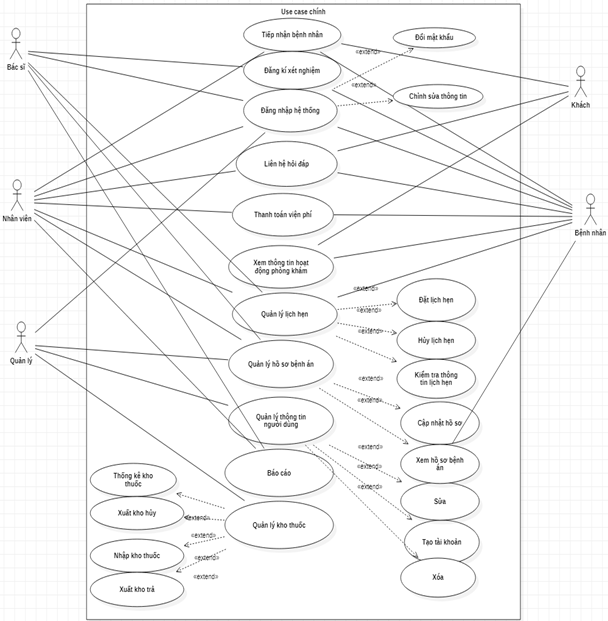
\includegraphics[scale=.8]{Hinh/Sơ đồ use case.png}
		\end{center}
		\caption{Sơ đồ Use Case tổng quát}
	\end{figure}
\end{center}

\pagebreak
\begin{center}
	\begin{figure}[!htp]
		\subsection{Sơ đồ Use Case Bệnh nhân}
		\begin{center}
			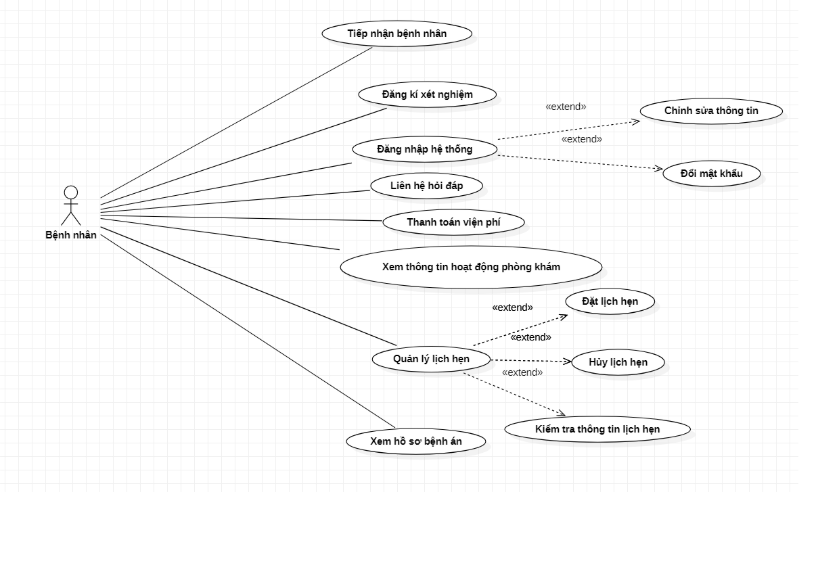
\includegraphics[scale=.6]{Hinh/Sơ đồ Use Case Bệnh nhân}
		\end{center}
		\caption{Sơ đồ Use Case Bệnh nhân}
	\end{figure}
\end{center}

\begin{center}
	\begin{figure}[!htp]
		\subsection{Sơ đồ Use Case Khách}
		\begin{center}
			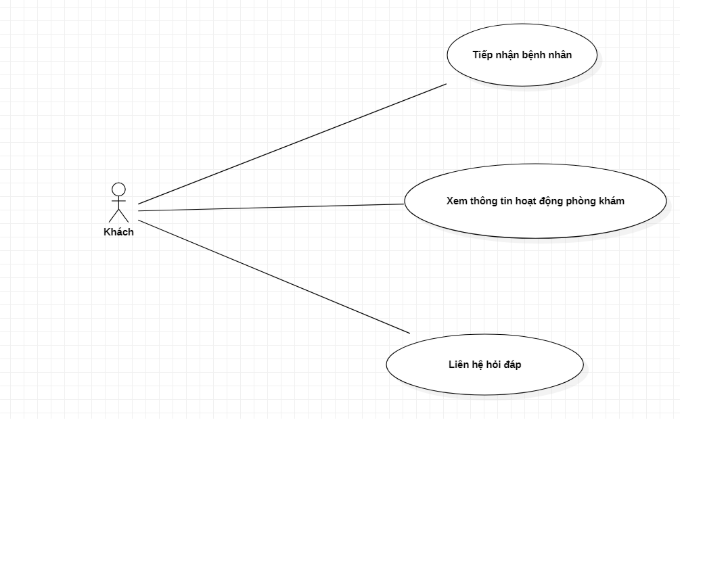
\includegraphics[scale=.7]{Hinh/Sơ đồ Use Case Khách.png}
		\end{center}
		\caption{Sơ đồ Use Case Khách}
	\end{figure}
\end{center}

\pagebreak
\begin{center}
	\begin{figure}[!htp]
		\subsection{Sơ đồ Use Case Nhân viên}
		\begin{center}
			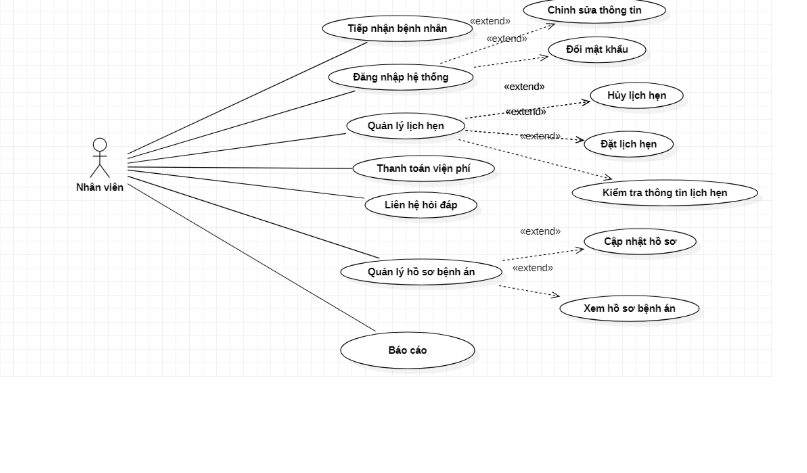
\includegraphics[scale=.6]{Hinh/Sơ đồ Use Case Nhân viên.png}
		\end{center}
		\caption{Sơ đồ Use Case Nhân viên}
	\end{figure}
\end{center}

\begin{center}
	\begin{figure}[!htp]
		\subsection{Sơ đồ Use Case Quản lý}
		\begin{center}
			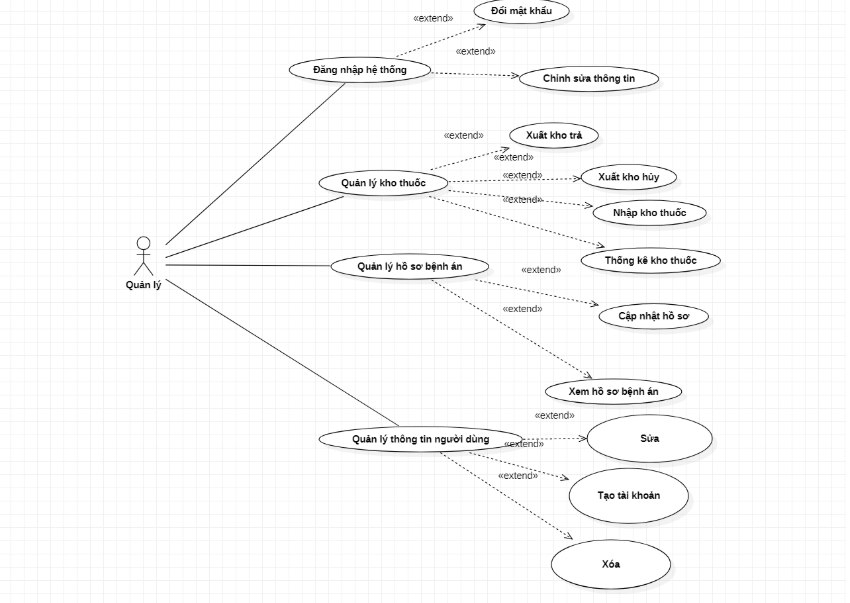
\includegraphics[scale=.5]{Hinh/Sơ đồ Use Case Quản lý.png}
		\end{center}
		\caption{Sơ đồ Use Case Quản lý}
	\end{figure}
\end{center}

\begin{center}
	\begin{figure}[!htp]
		\subsection{Sơ đồ Use Case Bác sĩ}
		\begin{center}
			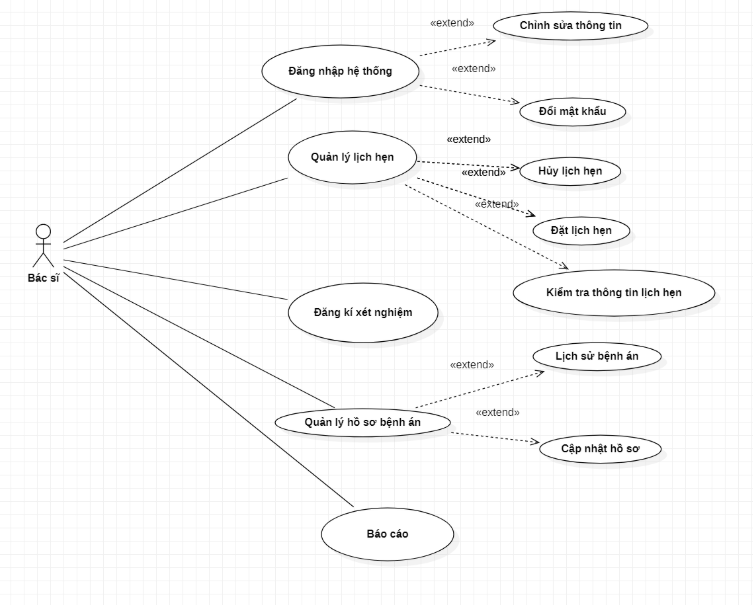
\includegraphics[scale=.6]{Hinh/Sơ đồ Use Case Bác sĩ.png}
		\end{center}
		\caption{Sơ đồ Use Case Bác sĩ}
	\end{figure}
\end{center}



\pagebreak
\section{Đặc tả Use Case}
\subsection{Use Case 1 : Tiếp nhận và ghi nhận thông tin bệnh nhân}
\centering
\begin{longtable}{|m{3cm}|m{14cm}|}
	\hline
		\centering\textbf{Tên Use Case} & Tiếp nhận thông tin bệnh nhân\\
	\hline
		\centering \textbf{Mô tả} & -Thông qua thông tin của bệnh nhân, nhân viên sẽ làm thủ tục tạo sổ cho bệnh nhân khám bệnh, nếu bệnh nhân chưa có đăng ký thông tin, nhân viên sẽ tạo mới thông tin và tiếp tục thủ tục tạo sổ hồ sơ bệnh án.\\ 
	\hline
		\centering \textbf{Tác nhân} & Nhân viên , bệnh nhân , khách\\ 
	\hline
		\centering \textbf{Sự kiện kích hoạt} & -Với tác nhân là bệnh nhân : nhân viên chọn “Xem thông tin bệnh nhân” sau đó sẽ điền thông tin vào sổ khám bệnh.
		\newline -Với tác nhân là khách : nhân viên chọn “Tạo thông tin bệnh nhân” để tạo mới thông tin bệnh nhân. \\ 
	\hline
		\centering \textbf{Điều kiện tiên quyết} & -Với tác nhân là nhân viên : có tài khoản do phòng khám cung cấp
		\newline -Với tác nhân là bệnh nhân : Đã lưu trữ thông tin bệnh nhân bởi phòng khám \\ 
	\hline
			\centering \textbf{Luồng sự kiện} & \begin{tabular}{|m{5cm}|m{7cm}|}
		\hline
			\centering \textbf{Tác nhân} & \centerline{\textbf{Hệ thống}} \\
		\hline
		1. Nhân viên chọn chức năng “Xem thông tin bệnh nhân” 
		\newline 2. Nhân viên điền thông tin vào sổ khám bệnh đồng thời lưu trữ lịch sử khám bệnh vào hệ thống. &
		1. Hiển thị thông tin bệnh nhân và lịch sử khám bệnh của bệnh nhân.
		\newline 2.Lưu trữ thêm lịch sử vào thông tin bệnh nhân\\
		\hline
	\end{tabular}\\
	\hline
	\centering \textbf{Kết quả} & -Tạo ra được sổ khám bệnh cho bệnh nhân\\ 
	\hline
	\centering \textbf{Ngoại lệ} & - Không\\ 
	\hline
	\caption{UC01 - Tiếp nhận và ghi nhận thông tin bệnh nhân}
\end{longtable}

\subsection{Use Case 2 : Đăng ký xét nghiệm}
\centering
\begin{longtable}{|m{3cm}|m{14cm}|}
	\hline
	\centering\textbf{Tên Use Case} & Đăng ký xét nghiệm\\
	\hline
	\centering \textbf{Mô tả} & Bệnh nhân có thể đăng kí xét nghiệm máu, chụp X-quang, siêu âm trước để tránh việc chờ đợi khi đến phòng khám, chức năng không dành cho khách.\\ 
	\hline
	\centering \textbf{Tác nhân} & Bác sĩ, bệnh nhân\\ 
	\hline
	\centering \textbf{Sự kiện kích hoạt} & Với tác nhân là bệnh nhân : chọn “Đăng ký xét nghiệm” sau đó sẽ điền thông tin vào phiếu đăng ký. \\ 
	\hline
	\centering \textbf{Điều kiện tiên quyết} & Phải là bệnh nhân thì mới có quyền đăng ký xét nghiệm, nếu là khách chưa thực hiện điều trị tại bệnh viện thì không có quyền đăng ký.\\ 
	\hline
	\centering \textbf{Luồng sự kiện} & \begin{tabular}{|m{5cm}|m{7cm}|}
		\hline
		\centering \textbf{Tác nhân} & \centerline{\textbf{Hệ thống}} \\
		\hline
		1. Bệnh nhân chọn chức năng “Đăng ký xét nghiệm” 
		\newline 2. Bệnh nhân điền thông tin vào phiếu đăng ký. &
		1. Hiển thị thông tin các mục của phiếu đăng ký.
		\newline 2. Thông tin phiếu đăng ký bệnh nhân đã điền sẽ được lưu trữ vào hệ thống để thực hiện xét nghiệm cho bệnh nhân.\\
		\hline
	\end{tabular}\\
	\hline
	\centering \textbf{Kết quả} & -Thông tin đăng ký sẽ được lưu vào hệ thống của bệnh viện, bệnh nhân sẽ được xét nghiệm.\\ 
	\hline
	\centering \textbf{Ngoại lệ} & - Không\\ 
	\hline
	\caption{UC02 - Đăng ký xét nghiệm}
\end{longtable}

\pagebreak
\subsection{Use Case 3 : Đăng nhập}
\centering
\begin{longtable}{|m{3cm}|m{14cm}|}
	\hline
		\centering\textbf{Tên Use Case} & Đăng nhập\\
	\hline
		\centering \textbf{Mô tả} & Nhân viên, quản lý, bác sĩ cần sử dụng tài khoản để truy cập vào hệ thống. Bệnh nhân cần xem hồ sơ bệnh án của bản thân\\ 
	\hline
		\centering \textbf{Tác nhân} & Quản lý, bác sĩ, nhân viên, bệnh nhân\\ 
	\hline
		\centering \textbf{Sự kiện kích hoạt} & - Quản lý, bác sĩ, nhân viên, bệnh nhân chọn nút “Đăng nhập”.\\ 
	\hline
		\centering \textbf{Điều kiện tiên quyết} & - Việc đăng nhập chỉ được thực hiện khi cần truy cập vào hệ thống và chỉ thành công khi tài khoản đã được tạo trước đó.\\ 
	\hline
		\centering \textbf{Luồng sự kiện} & \begin{tabular}{|m{5cm}|m{7cm}|}
		\hline
			\centering \textbf{Tác nhân} & \centerline{\textbf{Hệ thống}} \\
		\hline
			1. Nhập tài khoản và mật khẩu
			\newline 2. Chọn nút đăng nhập &
			 1. Giao diện đăng nhập
			 \newline 2. Kiểm tra tài khoản:
			 \newline 2.1. Thông báo nhập lại nếu thông tin không hợp lệ.
			 \newline 2.2. Kiểm tra thông tin đăng nhập
			 \newline 2.2.1. Thông báo khi sai thông tin đăng nhập với dữ liệu tài khoản trong cơ sở dữ liệu
			 \newline 2.2.2. Thông báo đăng nhập thành công nếu tài khoản hợp lệ.\\
		\hline
		\end{tabular}\\
	\hline
		\centering \textbf{Kết quả} & - Đăng nhập vào hệ thống thành công\\ 
	\hline
		\centering \textbf{Ngoại lệ} & - Không\\ 
	\hline
	\caption{UC03 - Đăng nhập}
\end{longtable}

\subsection{Use Case 4 : Lấy số thứ tự }
\centering
\begin{longtable}{|m{3cm}|m{14cm}|}
	\hline
	\centering\textbf{Tên Use Case} & Lấy số thứ tự \\
	\hline
	\centering \textbf{Mô tả} & Thông qua form lấy số thứ tự, bệnh nhân có thể bốc số thứ tự để khám, nếu là khách thì phải liên hệ với nhân viên để được tư vấn cũng như đăng ký thông tin bệnh nhân.\\ 
	\hline
	\centering \textbf{Tác nhân} & bệnh nhân, nhân viên\\ 
	\hline
	\centering \textbf{Sự kiện kích hoạt} & Sau khi đăng nhập vào hệ thống, chọn mục “Lấy số thứ tự”.\\ 
	\hline
	\centering \textbf{Điều kiện tiên quyết} & Phải đăng nhập bằng tài khoản của nhân viên hoặc bệnh nhân.\\ 
	\hline
	\centering \textbf{Điều kiện sau} & Mỗi người chỉ được lấy một số thứ tự cho một ngày\\ 
	\hline
	\centering \textbf{Luồng sự kiện} & \begin{tabular}{|m{5cm}|m{7cm}|}
		\hline
		\centering \textbf{Tác nhân} & \centerline{\textbf{Hệ thống}} \\
		\hline
				1. Đăng nhập vào hệ thống.
		\newline 2. Chọn chức năng “Lấy số thứ tự”.
		\newline 3. Tích "Booked" và chọn "Create".
		&
		1. Thực hiện xác thực đăng nhập.
		\newline 2. Hiển thị tên form xác nhận lấy số thứ tự.
		\newline 3. Hiển thị thông báo về số thứ tự của người dùng\\
		\hline
	\end{tabular}\\
	\hline
	\centering \textbf{Kết quả} & Hiển thị kết quả của số thứ tự\\ 
	\hline
	\centering \textbf{Ngoại lệ} & Nếu bệnh nhân đã có số thứ tự thì sẽ thông báo cho bệnh nhân và cho bệnh nhân biết về số thứ tự của mình.\\ 
	\hline
	\caption{UC04 - Lấy số thứ tự}
\end{longtable}


\subsection{Use Case 5 : Liên hệ hỏi đáp}
\centering
\begin{longtable}{|m{3cm}|m{14cm}|}
	\hline
	\centering\textbf{Tên Use Case} & Liên hệ hỏi đáp\\
	\hline
	\centering \textbf{Mô tả} & Nếu có những thắc mắc về bệnh lý cũng như dịch vụ của phòng khám, khách hoặc bệnh nhân có thể liên hệ hỏi đáp trực tuyến với nhân viên phòng khám.\\ 
	\hline
	\centering \textbf{Tác nhân} & Bệnh nhân, nhân viên, khách\\ 
	\hline
	\centering \textbf{Sự kiện kích hoạt} & -Với tác nhân là bệnh nhân hay khách: Sau khi đăng nhập vào hệ thống, chọn mục “Liên hệ hỏi đáp”.
	\newline -Với tác nhân là nhân viên: Nhân viên sẽ phải tiếp nhận tư vấn cho bệnh nhân và khách, giải đáp các thắc mắc về bệnh lý và dịch vụ cần thiết.
	\\ 
	\hline
	\centering \textbf{Điều kiện tiên quyết} & Phải đăng nhập bằng tài khoản nhân viên hoặc bệnh nhân.\\
	\hline
	\centering \textbf{Điều kiện sau} & Việc liên hệ phải trong thời gian làm việc của nhân viên.\\ 
	\hline
	\centering \textbf{Luồng sự kiện} & \begin{tabular}{|m{5cm}|m{7cm}|}
		\hline
		\centering \textbf{Tác nhân} & \centerline{\textbf{Hệ thống}} \\
		\hline
		1. Đăng nhập vào hệ thống.
		\newline 2. Chọn chức năng “Liên hệ hỏi đáp”.
		\newline 3. Nhập thông tin cần hỏi đáp để nhân viên có thể giải thích
		&
		1. Thực hiện xác thực đăng nhập.
		\newline 2. Hiển thị giao diện liên hệ hỏi đáp..
		\newline 3.  Kiểm tra và liên hệ tới tài khoản nhân viên.\\
		\hline
	\end{tabular}\\
	\hline
	\centering \textbf{Kết quả} & Hiển thị giao diện liên hệ hỏi đáp\\ 
	\hline
	\centering \textbf{Ngoại lệ} & Nếu bệnh nhân hay khách hỏi đáp không thành công, có thể sẽ do thời gian hỏi đáp không nằm trong thời gian làm việc của nhân viên.\\ 
	\hline
	\caption{UC05 - Liên hệ hỏi đáp}
\end{longtable}

\subsection{Use Case 6 : Tìm kiếm thông tin bệnh nhân}
\centering
\begin{longtable}{|m{3cm}|m{14cm}|}
	\hline
	\centering\textbf{Tên Use Case} & Tìm kiếm thông tin bệnh nhân\\
	\hline
	\centering \textbf{Mô tả} & Khi bác sĩ, quản lý, nhân viên muốn tìm kiếm thông tin của một bệnh nhân đã có trong database của bệnh viện.\\ 
	\hline
	\centering \textbf{Tác nhân} & Bác sĩ, quản lý, bệnh nhân, nhân viên\\ 
	\hline
	\centering \textbf{Sự kiện kích hoạt} & Khi bác sĩ hay quản lý chọn “Tìm kiếm bệnh nhân” trên hệ thống của bệnh viện.\\ 
	\hline
	\centering \textbf{UC liên quan} & Đăng nhập\\ 
	\hline
	\centering \textbf{Điều kiện tiên quyết} & Phải đăng nhập bằng tài khoản của bác sĩ,nhân viên hoặc quản lý của bệnh viện.\\
	\hline
	\centering \textbf{Điều kiện sau} & Đăng nhập thành công\\ 
	\hline
	\centering \textbf{Luồng sự kiện} & \begin{tabular}{|m{5cm}|m{7cm}|}
		\hline
		\centering \textbf{Tác nhân} & \centerline{\textbf{Hệ thống}} \\
		\hline
		1. Đăng nhập vào hệ thống.
		\newline 2. Chọn chức năng “Tìm kiếm bệnh nhân”.
		\newline 3. Nhập tên bệnh nhân hoặc những thông tin có liên quan vào thanh được hiển thị. Sau đó chọn “Tìm kiếm” 
		&
		1. Thực hiện xác thực đăng nhập.
		\newline 2. Hiển thị thanh tìm kiếm.
		\newline 3. Kiểm tra và xuất thông tin về bệnh nhân được tìm kiếm.\\
		\hline
	\end{tabular}\\
	\hline
	\centering \textbf{Kết quả} & Hiển thị ra thông tin của bệnh nhân dựa vào kết quả tìm kiếm.\\ 
	\hline
	\centering \textbf{Ngoại lệ} & Nếu thông tin không có trong database của bệnh viện thì sẽ không có thông tin nào được hiển thị.\\ 
	\hline
	\caption{UC06 - Tìm kiếm thông tin bệnh nhân}
\end{longtable}

\subsection{Use Case 7 : Thanh toán viện phí}
\centering
\begin{longtable}{|m{3cm}|m{14cm}|}
	\hline
	\centering\textbf{Tên Use Case} & Thanh toán viện phí\\
	\hline
	\centering \textbf{Mô tả} & Sau khi bệnh nhân khám bệnh hoàn tất và không có nhu cầu khám thêm, bệnh nhân có thể kiểm tra thông tin viện phí trong hồ sơ bệnh án.\\ 
	\hline
	\centering \textbf{Tác nhân} & Nhân viên, bệnh nhân\\ 
	\hline
	\centering \textbf{Sự kiện kích hoạt} & Khi chọn chức năng “Thanh toán viện phí” ở trên hệ thống của bệnh viện.\\ 
	\hline
	\centering \textbf{UC liên quan} & Đăng nhập, Tìm kiếm thông tin bệnh nhân\\ 
	\hline
	\centering \textbf{Điều kiện tiên quyết} & Phải đăng nhập thành công và tìm được thông tin bệnh nhân muốn thanh toán viện phí.\\
	\hline
	\centering \textbf{Luồng sự kiện} & \begin{tabular}{|m{5cm}|m{7cm}|}
		\hline
		\centering \textbf{Tác nhân} & \centerline{\textbf{Hệ thống}} \\
		\hline
		1. Đăng nhập vào hệ thống.
		\newline 2. Thực hiện chức năng “Tìm kiếm”, sau đó chọn chức năng “Thanh toán viện phí”
		\newline 3. Nhập số tiền bệnh nhân đã thanh toán và chọn “Submit”.
		\newline 4. Xác thực mật khẩu.
		&
		1.1 Thực hiện việc xác thực đăng nhập.
		\newline 2.1 Hiển thị thông tin về viện phí của bệnh nhân đó.	
		\newline 3.1 Hiện xác thực lại bằng mật khẩu.
		\newline 4.1 Thông báo thành công nếu xác thực thành công. Thông tin vừa thực hiện sẽ được lưu vào database.
		\\
		\hline
	\end{tabular}\\
	\hline
	\centering \textbf{Kết quả} & Hệ thống sẽ được cập nhật và hiển thị “Thanh toán thành công”.\\ 
	\hline
	\centering \textbf{Ngoại lệ} & Không có.\\ 
	\hline
	\caption{UC07 - Thanh toán viện phí}
\end{longtable}

\subsection{Use Case 8 : Xem thông tin, hoạt động phòng khám}
\centering
\begin{longtable}{|m{3cm}|m{14cm}|}
	\hline
	\centering\textbf{Tên Use Case} & Xem thông tin, hoạt động phòng khám\\
	\hline
	\centering \textbf{Mô tả} & Các hoạt động, dịch vụ, sửa chữa, bảo trì,.. phòng khám được đăng lên cổng thông tin trực tuyến Trang Chủ của phòng khám để khách cũng như bệnh nhân tiện theo dõi các hoạt động.\\ 
	\hline
	\centering \textbf{Tác nhân} & Bệnh nhân, khách\\ 
	\hline
	\centering \textbf{Sự kiện kích hoạt} & Truy cập vào cổng thông tin trực tuyến Trang Chủ của phòng khám.\\ 
	\hline
	\centering \textbf{Điều kiện tiên quyết} & Phải là trang chủ phòng khám mà bệnh nhân hay khách cần xem.\\
	\hline
	\centering \textbf{Luồng sự kiện} & \begin{tabular}{|m{5cm}|m{7cm}|}
		\hline
		\centering \textbf{Tác nhân} & \centerline{\textbf{Hệ thống}} \\
		\hline
		1. Truy cập vào trang chủ của phòng khám.
		\newline2. Chọn các dịch vụ hay thông báo cần xem.
		&
		1. Hiển thị giao diện trang chủ.	
		\newline 2. Hiển thị giao diện các dịch vụ, thông báo mà tác nhân đã chọn.\\
		\hline
	\end{tabular}\\
	\hline
	\centering \textbf{Kết quả} & Hiển thị giao diện các dịch vụ, thông tin hoạt động của phòng khám.\\ 
	\hline
	\centering \textbf{Ngoại lệ} & Không.\\ 
	\hline
	\caption{UC08 - Xem thông tin, hoạt động phòng khám}
\end{longtable}

\subsection{Use Case 9 : Xem tổng quát, chi tiết tất cả hồ sơ bệnh án}
\centering
\begin{longtable}{|m{3cm}|m{14cm}|}
	\hline
	\centering\textbf{Tên Use Case} & Xem tổng quát, chi tiết tất cả hồ sơ bệnh án\\
	\hline
	\centering \textbf{Mô tả} & Thông qua chức năng quản lý: quản lý có thể xem được tất cả lịch sử bệnh án của mọi bệnh nhân, các chi tiết về hồ sơ của bệnh nhân.\\ 
	\hline
	\centering \textbf{Tác nhân} & Bác sĩ, quản lý, nhân viên.\\ 
	\hline
	\centering \textbf{Sự kiện kích hoạt} & Đăng nhập vào hệ thống và chọn chức năng “Các hồ sơ bệnh án”.\\ 
	\hline
	\centering \textbf{Điều kiện tiên quyết} & Đăng nhập bằng tài khoản của bác sĩ, quản lý hoặc nhân viên.\\
	\hline
	\centering \textbf{Điều kiện sau} & Đăng nhập thành công.\\
	\hline
	\centering \textbf{Luồng sự kiện} & \begin{tabular}{|m{5cm}|m{7cm}|}
		\hline
		\centering \textbf{Tác nhân} & \centerline{\textbf{Hệ thống}} \\
		\hline	
		1.Đăng nhập vào hệ thống.
		\newline 2.Chọn mục xem Hồ sơ bệnh án.	
		&
		1.Thực hiện việc xác thực đăng nhập.
		\newline 2.Hiển thị giao diện hồ sơ bệnh án của tất cả bệnh nhân.
		\\
		\hline
	\end{tabular}\\
	\hline
	\centering \textbf{Kết quả} & Hệ thống hiển thị giao diện tất cả hồ sơ bệnh án của các bệnh nhân.\\ 
	\hline
	\centering \textbf{Ngoại lệ} & Không có.\\ 
	\hline
	\caption{UC09 - Xem tổng quát, chi tiết tất cả hồ sơ bệnh án}
\end{longtable}

\subsection{Use Case 10 : Xem hồ sơ bệnh án}
\centering
\begin{longtable}{|m{3cm}|m{14cm}|}
	\hline
	\centering\textbf{Tên Use Case} & Xem hồ sơ bệnh án\\
	\hline
	\centering \textbf{Mô tả} & Khi bệnh nhân đến khám bệnh, bác sĩ sẽ truy cập vào hồ sơ của bệnh nhân để có thể xem được: lịch sử bệnh án, bệnh án đang điều trị, bệnh án đang chờ kết quả xét nghiệm,...\\ 
	\hline
	\centering \textbf{Tác nhân} & Bác sĩ, bệnh nhân.\\ 
	\hline
	\centering \textbf{Sự kiện kích hoạt} & Đăng nhập vào hệ thống và chọn chức năng “Các hồ sơ bệnh án”, sau đó chọn “Xem hồ sơ bệnh án” của bệnh nhân cần xem.\\ 
	\hline
	\centering \textbf{Điều kiện tiên quyết} & Đăng nhập bằng tài khoản của bác sĩ.\\
	\hline
	\centering \textbf{Điều kiện sau} & Đăng nhập thành công.\\
	\hline
	\centering \textbf{Luồng sự kiện} & \begin{tabular}{|m{5cm}|m{7cm}|}
		\hline
		\centering \textbf{Tác nhân} & \centerline{\textbf{Hệ thống}} \\
		\hline	
		1.Đăng nhập vào hệ thống.
		\newline 2.Chọn mục xem Hồ sơ bệnh án.
		\newline 3.Chọn hồ sơ bệnh án của của bệnh nhân mà bác sĩ cần xem.
		&
		1.Thực hiện việc xác thực đăng nhập.
		\newline 2.Hiển thị giao diện danh sách hồ sơ bệnh án của tất cả bệnh nhân.
		\newline 3.Hiển thị giao diện hồ sơ bệnh án của bệnh nhân đã chọn.\\
		\hline
	\end{tabular}\\
	\hline
	\centering \textbf{Kết quả} & Hệ thống hiển thị giao diện hồ sơ bệnh án của bệnh nhân.\\ 
	\hline
	\centering \textbf{Ngoại lệ} & Không có.\\ 
	\hline
	\caption{UC10 - Xem hồ sơ bệnh án}
\end{longtable}


\subsection{Use Case 11 : Cập nhật hồ sơ bệnh án}
\centering
\begin{longtable}{|m{3cm}|m{14cm}|}
	\hline
	\centering\textbf{Tên Use Case} & Cập nhật hồ sơ bệnh án\\
	\hline
	\centering \textbf{Mô tả} & Sau khi hoàn tất trong những giai đoạn khám bệnh cho bệnh nhân, bác sĩ có nhiệm vụ phải cập nhật quy trình điều trị, thời gian điều trị, thuốc điều trị vào trong hồ sơ bệnh án của bệnh nhân để theo dõi và điều trị bệnh.\\ 
	\hline
	\centering \textbf{Tác nhân} & Bác sĩ.\\ 
	\hline
	\centering \textbf{Sự kiện kích hoạt} & Đăng nhập vào hệ thống và chọn chức năng “Xem hồ sơ bệnh án” của bệnh nhân đã hoàn tất giai đoạn khám bệnh, sau đó chọn “Cập nhật hồ sơ bệnh án”.\\ 
	\hline
	\centering \textbf{Điều kiện tiên quyết} & Đăng nhập bằng tài khoản của bác sĩ.\\
	\hline
	\centering \textbf{Điều kiện sau} & Đăng nhập thành công.\\
	\hline
	\centering \textbf{Luồng sự kiện} & \begin{tabular}{|m{5cm}|m{7cm}|}
		\hline
		\centering \textbf{Tác nhân} & \centerline{\textbf{Hệ thống}} \\
		\hline	
		1.Đăng nhập vào hệ thống.
		\newline 2.Chọn hồ sơ bệnh án của bệnh nhân mà bác sĩ cần cập nhật.
		\newline 3.Chọn cập nhật hồ sơ bệnh án.
		&
		1.Thực hiện việc xác thực đăng nhập.
		\newline 2.Hiển thị giao diện hồ sơ bệnh án của bệnh nhân đã chọn.
		\newline 3.Hiển thị giao diện các thông tin cần cập nhật và chỉnh sửa.\\
		\hline
	\end{tabular}\\
	\hline
	\centering \textbf{Kết quả} & Hệ thống hiển thị giao diện cập nhật hồ sơ bệnh án của bệnh nhân.\\ 
	\hline
	\centering \textbf{Ngoại lệ} & Không có.\\ 
	\hline
	\caption{UC11 - Cập nhật hồ sơ bệnh án}
\end{longtable}

\pagebreak
\subsection{Use Case 12 : Xem thông tin kho thuốc}
\centering
\begin{longtable}{|m{3cm}|m{14cm}|}
	\hline
	\centering\textbf{Tên Use Case} & Xem thông tin kho thuốc\\
	\hline
	\centering \textbf{Mô tả} & Nhân viên có nhiệm vụ phải sắp xếp lịch hẹn giữa bệnh nhân và bác sĩ và thông báo cho bác sĩ hoặc bệnh nhân nếu bác sĩ hoặc bệnh nhân hủy lịch hẹn.\\ 
	\hline
	\centering \textbf{Tác nhân} & Quản lý.\\ 
	\hline
	\centering \textbf{Sự kiện kích hoạt} & Đăng nhập vào hệ thống, sau đó chọn “Xem thông tin kho thuốc”.\\ 
	\hline
	\centering \textbf{Điều kiện tiên quyết} & Phải đăng nhập bằng tài khoản của quản lý.\\
	\hline
	\centering \textbf{Luồng sự kiện} & \begin{tabular}{|m{5cm}|m{7cm}|}
		\hline
		\centering \textbf{Tác nhân} & \centerline{\textbf{Hệ thống}} \\
		\hline	
		1. Đăng nhập vào hệ thống.
		\newline 2. Chọn chức năng “Xem thông tin kho thuốc”.
		&
		1. Thực hiện xác thực đăng nhập.
		\newline 2. Hiển thị giao diện thông tin kho thuốc.
		\\
		\hline
	\end{tabular}\\
	\hline
	\centering \textbf{Kết quả} & Hiển thị giao diện thông tin kho thuốc.\\ 
	\hline
	\centering \textbf{Ngoại lệ} & Không.\\ 
	\hline
	\caption{UC12 - Xem thông tin kho thuốc}
\end{longtable}

\subsection{Use Case 13 : Thống kê kho thuốc}
\centering
\begin{longtable}{|m{3cm}|m{14cm}|}
	\hline
	\centering\textbf{Tên Use Case} & Thống kê kho thuốc\\
	\hline
	\centering \textbf{Mô tả} & Hàng tháng, nhân viên sẽ điền vào form báo cáo, bao gồm: số thuốc nhập đầu tháng, số thuốc còn tồn trong kho cuối tháng, số thuốc hết hạn ở kho.\\ 
	\hline
	\centering \textbf{Tác nhân} & Quản lý, nhân viên.\\ 
	\hline
	\centering \textbf{Sự kiện kích hoạt} & Đăng nhập vào hệ thống, sau đó chọn “Thống kê kho thuốc”.\\ 
	\hline
	\centering \textbf{Điều kiện tiên quyết} & Phải đăng nhập bằng tài khoản của quản lý hoặc nhân viên.\\
	\hline
	\centering \textbf{Luồng sự kiện} & \begin{tabular}{|m{5cm}|m{7cm}|}
		\hline
		\centering \textbf{Tác nhân} & \centerline{\textbf{Hệ thống}} \\
		\hline	
		1. Đăng nhập vào hệ thống.
		\newline 2. Chọn chức năng “Thống kê kho thuốc”.
		\newline 3.Nhập các thông tin của kho thuốc trong form báo cáo.
		\newline 4.Submit.
		&
		1. Thực hiện xác thực đăng nhập.
		\newline 2. Hiển thị giao diện thống kê kho thuốc.
		\newline 3.Hiển thị form báo cáo thống kê kho thuốc.
		\newline 4.Kiểm tra và xuất kết quả submit thành công.
		\\
		\hline
	\end{tabular}\\
	\hline
	\centering \textbf{Kết quả} & Hiển thị kết quả thống kê thành công.\\ 
	\hline
	\centering \textbf{Ngoại lệ} & Nếu không thống kê thành công thì sẽ là do nhân viên chưa nhập đầy đủ thông tin cần thống kê.\\ 
	\hline
	\caption{UC13 - Thống kê kho thuốc}
\end{longtable}

\subsection{Use Case 14 : Nhập kho thuốc}
\centering
\begin{longtable}{|m{3cm}|m{14cm}|}
	\hline
	\centering\textbf{Tên Use Case} & Nhập kho thuốc\\
	\hline
	\centering \textbf{Mô tả} & Bác sĩ và nhân viên có thể gửi yêu cầu nhập kho thuốc ở trong tháng nếu số lượng thuốc trong kho đã hết hoặc nhu cầu sử dụng thuốc để trị bệnh cho bệnh nhân lên cao.\\ 
	\hline
	\centering \textbf{Tác nhân} & Quản lý, nhân viên, bác sĩ.\\ 
	\hline
	\centering \textbf{Sự kiện kích hoạt} & Đăng nhập vào hệ thống, sau đó chọn “Nhập kho thuốc”.\\ 
	\hline
	\centering \textbf{Điều kiện tiên quyết} & Phải đăng nhập bằng tài khoản của quản lý, bác sĩ hoặc nhân viên.\\
	\hline
	\centering \textbf{Luồng sự kiện} & \begin{tabular}{|m{5cm}|m{7cm}|}
		\hline
		\centering \textbf{Tác nhân} & \centerline{\textbf{Hệ thống}} \\
		\hline	
		1. Đăng nhập vào hệ thống.
		\newline 2. Chọn chức năng “Nhập kho thuốc”.
		\newline 3.Gửi yêu cầu nhập kho thuốc
		&
		1. Thực hiện xác thực đăng nhập.
		\newline 2. Hiển thị giao diện nhập kho thuốc.
		\newline 3.Hệ thống gửi yêu cầu nhập kho thuốc tới tài khoản của quản lý.
		\\
		\hline
	\end{tabular}\\
	\hline
	\centering \textbf{Kết quả} & Hệ thống gửi yêu cầu nhập kho thuốc của nhân viên, bác sĩ tới quản lý.\\ 
	\hline
	\centering \textbf{Ngoại lệ} & Không.\\ 
	\hline
	\caption{UC14 - Nhập kho thuốc}
\end{longtable}

\subsection{Use Case 15 : Xuất kho trả}
\centering
\begin{longtable}{|m{3cm}|m{14cm}|}
	\hline
	\centering\textbf{Tên Use Case} & Xuất kho trả\\
	\hline
	\centering \textbf{Mô tả} & Khi nhân viên kiểm tra số thuốc vừa nhập mà không phải hoặc sai thuốc thì sẽ gửi yêu cầu trả lại kho.\\ 
	\hline
	\centering \textbf{Tác nhân} & Quản lý, nhân viên.\\ 
	\hline
	\centering \textbf{Sự kiện kích hoạt} & Đăng nhập vào hệ thống, sau đó chọn “Xuất kho trả”.\\ 
	\hline
	\centering \textbf{Điều kiện tiên quyết} & Phải đăng nhập bằng tài khoản của quản lý hoặc nhân viên.\\
	\hline
	\centering \textbf{Luồng sự kiện} & \begin{tabular}{|m{5cm}|m{7cm}|}
		\hline
		\centering \textbf{Tác nhân} & \centerline{\textbf{Hệ thống}} \\
		\hline	
		1. Đăng nhập vào hệ thống.
		\newline 2. Chọn chức năng “Xuất kho thuốc”.
		\newline 3.Gửi yêu xuất nhập kho thuốc
		&
		1. Thực hiện xác thực đăng nhập.
		\newline 2. Hiển thị giao diện nhập kho thuốc.
		\newline 3.Hệ thống gửi yêu cầu xuất kho thuốc tới tài khoản của quản lý.
		\\
		\hline
	\end{tabular}\\
	\hline
	\centering \textbf{Kết quả} & Hệ thống gửi yêu cầu xuất kho trả thuốc của nhân viên tới quản lý\\ 
	\hline
	\centering \textbf{Ngoại lệ} & Không.\\ 
	\hline
	\caption{UC15 - Xuất kho trả}
\end{longtable}

\subsection{Use Case 16 : Xuất kho hủy}
\centering
\begin{longtable}{|m{3cm}|m{14cm}|}
	\hline
	\centering\textbf{Tên Use Case} & Xuất kho hủy\\
	\hline
	\centering \textbf{Mô tả} & Khi nhân viên kiểm tra số thuốc vừa nhập từ đơn vị kho mà thuốc đã quá hạn sử dụng hoặc hư hỏng thì sẽ gửi yêu cầu hủy thuốc tới kho.\\ 
	\hline
	\centering \textbf{Tác nhân} & Quản lý, nhân viên.\\ 
	\hline
	\centering \textbf{Sự kiện kích hoạt} & Đăng nhập vào hệ thống, sau đó chọn “Xuất kho hủy”.\\ 
	\hline
	\centering \textbf{Điều kiện tiên quyết} & Phải đăng nhập bằng tài khoản của quản lý hoặc nhân viên.\\
	\hline
	\centering \textbf{Luồng sự kiện} & \begin{tabular}{|m{5cm}|m{7cm}|}
		\hline
		\centering \textbf{Tác nhân} & \centerline{\textbf{Hệ thống}} \\
		\hline	
		1. Đăng nhập vào hệ thống.
		\newline 2. Chọn chức năng “Xuất kho hủy”.
		\newline 3.Gửi yêu xuất kho hủy thuốc
		&
		1. Thực hiện xác thực đăng nhập.
		\newline 2. Hiển thị giao diện xuất kho hủy thuốc.
		\newline 3.Hệ thống gửi yêu cầu hủy thuốc tới tài khoản của quản lý.
		\\
		\hline
	\end{tabular}\\
	\hline
	\centering \textbf{Kết quả} & Hệ thống gửi yêu cầu hủy thuốc của nhân viên tới quản lý\\ 
	\hline
	\centering \textbf{Ngoại lệ} & Không.\\ 
	\hline
	\caption{UC16 - Xuất kho hủy}
\end{longtable}

\subsection{Use Case 17 : Báo cáo}
\centering
\begin{longtable}{|m{3cm}|m{14cm}|}
	\hline
	\centering\textbf{Tên Use Case} & Báo cáo\\
	\hline
	\centering \textbf{Mô tả} & Hằng tuần, tất cả nhân viên, điều dưỡng, y tá, bác sĩ sẽ báo cáo tình hình làm việc trên hệ thống và được gửi về quản lý.\\ 
	\hline
	\centering \textbf{Tác nhân} & Nhân viên, bác sĩ.\\ 
	\hline
	\centering \textbf{Sự kiện kích hoạt} & Đăng nhập vào hệ thống, sau đó chọn “Xuất kho hủy”.\\ 
	\hline
	\centering \textbf{Điều kiện tiên quyết} & Phải đăng nhập bằng tài khoản của bác sĩ hoặc nhân viên.\\
	\hline
	\centering \textbf{Luồng sự kiện} & \begin{tabular}{|m{5cm}|m{7cm}|}
		\hline
		\centering \textbf{Tác nhân} & \centerline{\textbf{Hệ thống}} \\
		\hline	
		1. Đăng nhập vào hệ thống.
		\newline 2. Chọn chức năng “Báo cáo”.
		\newline 3.Báo cáo tình hình làm việc và submit.
		&
		1. Thực hiện xác thực đăng nhập.
		\newline 2. Hiển thị báo cáo.
		\newline 3.Hệ thống kiểm tra và gửi báo cáo đã submit tới quản lý.
		\\
		\hline
	\end{tabular}\\
	\hline
	\centering \textbf{Kết quả} & Hệ thống gửi báo cáo đã submit của bác sĩ và nhân viên tới quản lý.\\ 
	\hline
	\centering \textbf{Ngoại lệ} & Không.\\ 
	\hline
	\caption{UC17 - Báo cáo}
\end{longtable}

\subsection{Use Case 18 : Xem thông tin người dùng}
\centering
\begin{longtable}{|m{3cm}|m{14cm}|}
	\hline
	\centering\textbf{Tên Use Case} & Xem thông tin người dùng\\
	\hline
	\centering \textbf{Mô tả} & Quản lý có thể xem được các nội dung bao gồm: thông tin chi tiết của bác sĩ, thông tin chi tiết của nhân viên, thông tin chi tiết của bệnh nhân.\\ 
	\hline
	\centering \textbf{Tác nhân} & Quản lý.\\ 
	\hline
	\centering \textbf{Sự kiện kích hoạt} & Sau khi đăng nhập vào hệ thống, chọn mục “Xem thông tin người dùng”.\\ 
	\hline
	\centering \textbf{Điều kiện tiên quyết} & Phải đăng nhập bằng tài khoản của quản lý.\\
	\hline
	\centering \textbf{Luồng sự kiện} & \begin{tabular}{|m{5cm}|m{7cm}|}
		\hline
		\centering \textbf{Tác nhân} & \centerline{\textbf{Hệ thống}} \\
		\hline	
		1. Đăng nhập vào hệ thống.
		\newline 2. Chọn chức năng “Xem thông tin người dùng”.
		&
		1. Thực hiện xác thực đăng nhập.
		\newline 2. Hiển thị giao diện thông tin người dùng.
		\\
		\hline
	\end{tabular}\\
	\hline
	\centering \textbf{Kết quả} & Hiển thị giao diện thông tin người dùng.\\ 
	\hline
	\centering \textbf{Ngoại lệ} & Không.\\ 
	\hline
	\caption{UC18 - Xem thông tin người dùng}
\end{longtable}

\subsection{Use Case 19 : Tạo tài khoản nhân viên}
\centering
\begin{longtable}{|m{3cm}|m{14cm}|}
	\hline
	\centering\textbf{Tên Use Case} & Tạo tài khoản nhân viên\\
	\hline
	\centering \textbf{Mô tả} & Quản lý thêm thông tin của người dùng cần được lưu vào hệ thống..\\ 
	\hline
	\centering \textbf{Tác nhân} & Quản lý.\\ 
	\hline
	\centering \textbf{Sự kiện kích hoạt} & Sau khi đăng nhập vào hệ thống, chọn mục “Tạo tài khoản nhân viên”.\\ 
	\hline
	\centering \textbf{Điều kiện tiên quyết} & Phải đăng nhập bằng tài khoản của quản lý.\\
	\hline
	\centering \textbf{Luồng sự kiện} & \begin{tabular}{|m{5cm}|m{7cm}|}
		\hline
		\centering \textbf{Tác nhân} & \centerline{\textbf{Hệ thống}} \\
		\hline	
		1. Đăng nhập vào hệ thống.
		\newline 2. Chọn chức năng “Tạo tài khoản nhân viên”.
		\newline 3.Submit
		&
		1. Thực hiện xác thực đăng nhập.
		\newline 2. Hiển thị giao diện tạo tài khoản nhân viên.
		\newline 3.Kiểm tra và lưu tài khoản nhân viên đã thêm vào database.
		\\
		\hline
	\end{tabular}\\
	\hline
	\centering \textbf{Kết quả} & Thêm tài khoản nhân viên vào hệ thống thành công.\\ 
	\hline
	\centering \textbf{Ngoại lệ} & Không.\\ 
	\hline
	\caption{UC19 - Tạo tài khoản nhân viên}
\end{longtable}

\subsection{Use Case 20 : Xóa thông tin người dùng}
\centering
\begin{longtable}{|m{3cm}|m{14cm}|}
	\hline
	\centering\textbf{Tên Use Case} & Xóa thông tin người dùng\\
	\hline
	\centering \textbf{Mô tả} & Quản lý xóa thông tin của người dùng khi người dùng vi phạm các điều luật hoặc người dùng không còn sử dụng hệ thống (thông tin sẽ được lưu vào bộ nhớ xóa).\\ 
	\hline
	\centering \textbf{Tác nhân} & Quản lý.\\ 
	\hline
	\centering \textbf{Sự kiện kích hoạt} & Sau khi đăng nhập vào hệ thống, chọn mục “Xem thông tin người dùng”, sau đó chọn “Xóa tài khoản người dùng”.\\ 
	\hline
	\centering \textbf{Điều kiện tiên quyết} & Phải đăng nhập bằng tài khoản của quản lý.\\
	\hline
	\centering \textbf{Luồng sự kiện} & \begin{tabular}{|m{5cm}|m{7cm}|}
		\hline
		\centering \textbf{Tác nhân} & \centerline{\textbf{Hệ thống}} \\
		\hline	
		1. Đăng nhập vào hệ thống.
		\newline 2. Chọn chức năng “Xem thông tin người dùng”.
		\newline 3.Chọn “Xóa tài khoản người dùng”
		&
		1. Thực hiện xác thực đăng nhập.
		\newline 2. Hiển thị giao diện tạo tài khoản người dùng.
		\newline 3.Kiểm tra và lưu tài khoản người dùng đã xóa vào bộ nhớ xóa.
		\\
		\hline
	\end{tabular}\\
	\hline
	\centering \textbf{Kết quả} & Lưu tài khoản người dùng đã xóa vào bộ nhớ xóa thành công.\\ 
	\hline
	\centering \textbf{Ngoại lệ} & Không.\\ 
	\hline
	\caption{UC20 - Xóa thông tin người dùng}
\end{longtable}

\subsection{Use Case 21 : Sửa thông tin người dùng}
\centering
\begin{longtable}{|m{3cm}|m{14cm}|}
	\hline
	\centering\textbf{Tên Use Case} & Sửa thông tin người dùng\\
	\hline
	\centering \textbf{Mô tả} & Quản lý sửa thông tin của người dùng khi thông tin cung cấp chưa chính xác hoặc cần thay đổi.\\ 
	\hline
	\centering \textbf{Tác nhân} & Quản lý.\\ 
	\hline
	\centering \textbf{Sự kiện kích hoạt} & Sau khi đăng nhập vào hệ thống, chọn mục “Xem thông tin người dùng”, sau đó chọn “Sửa tài khoản người dùng”.\\ 
	\hline
	\centering \textbf{Điều kiện tiên quyết} & Phải đăng nhập bằng tài khoản của quản lý.\\
	\hline
	\centering \textbf{Luồng sự kiện} & \begin{tabular}{|m{5cm}|m{7cm}|}
		\hline
		\centering \textbf{Tác nhân} & \centerline{\textbf{Hệ thống}} \\
		\hline	
		1. Đăng nhập vào hệ thống.
		\newline 2. Chọn chức năng “Xem thông tin người dùng”.
		\newline 3.Chọn “Sửa thông tin người dùng”.
		\newline 4.Submit
		&
		1. Thực hiện xác thực đăng nhập.
		\newline 2. Hiển thị giao diện tạo tài khoản người dùng.
		\newline 3.Hiển thị giao diện sửa tài khoản người dùng. 
		\newline 3.Kiểm tra và lưu tài khoản người dùng đã sửa vào hệ thống.
		\\
		\hline
	\end{tabular}\\
	\hline
	\centering \textbf{Kết quả} & Lưu tài khoản người dùng đã sửa vào hệ thống thành công.\\ 
	\hline
	\centering \textbf{Ngoại lệ} & Không.\\ 
	\hline
	\caption{UC21 - Sửa thông tin người dùng}
\end{longtable}

\pagebreak
\raggedright
\section{Sequence Diagram}
\begin{center}
	\begin{figure}[!htp]
		\subsection{Squence Diagram - Tiếp nhận và ghi nhận thông tin bệnh nhân}
		\begin{center}
			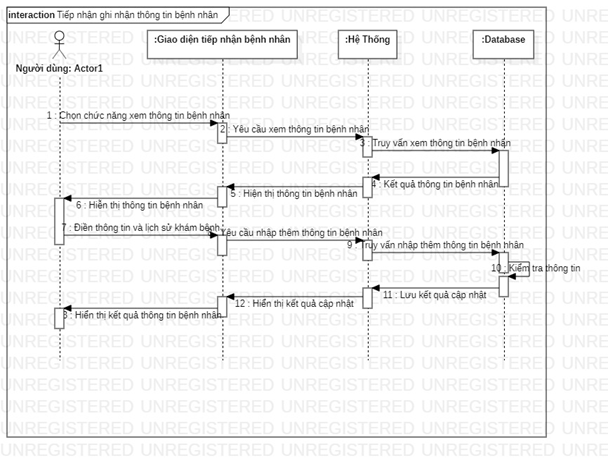
\includegraphics[scale=1]{Hinh/Sequence diagram Tiếp nhận và ghi nhận thông tin bệnh nhân.png}
		\end{center}
		\caption{Squence Diagram - Tiếp nhận và ghi nhận thông tin bệnh nhân}
	\end{figure}
\end{center}

\pagebreak
\begin{center}
	\begin{figure}[!htp]
		\subsection{Squence Diagram - Đăng ký xét nghiệm}
		\begin{center}
			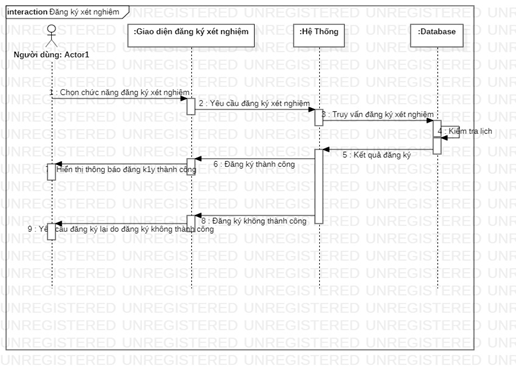
\includegraphics[scale=1]{Hinh/Sequence diagram Đăng ký xét nghiệm.png}
		\end{center}
		\caption{Squence Diagram - Đăng ký xét nghiệm}
	\end{figure}
\end{center}

\begin{center}
	\begin{figure}[!htp]
		\subsection{Squence Diagram - Đăng nhập}
		\begin{center}
			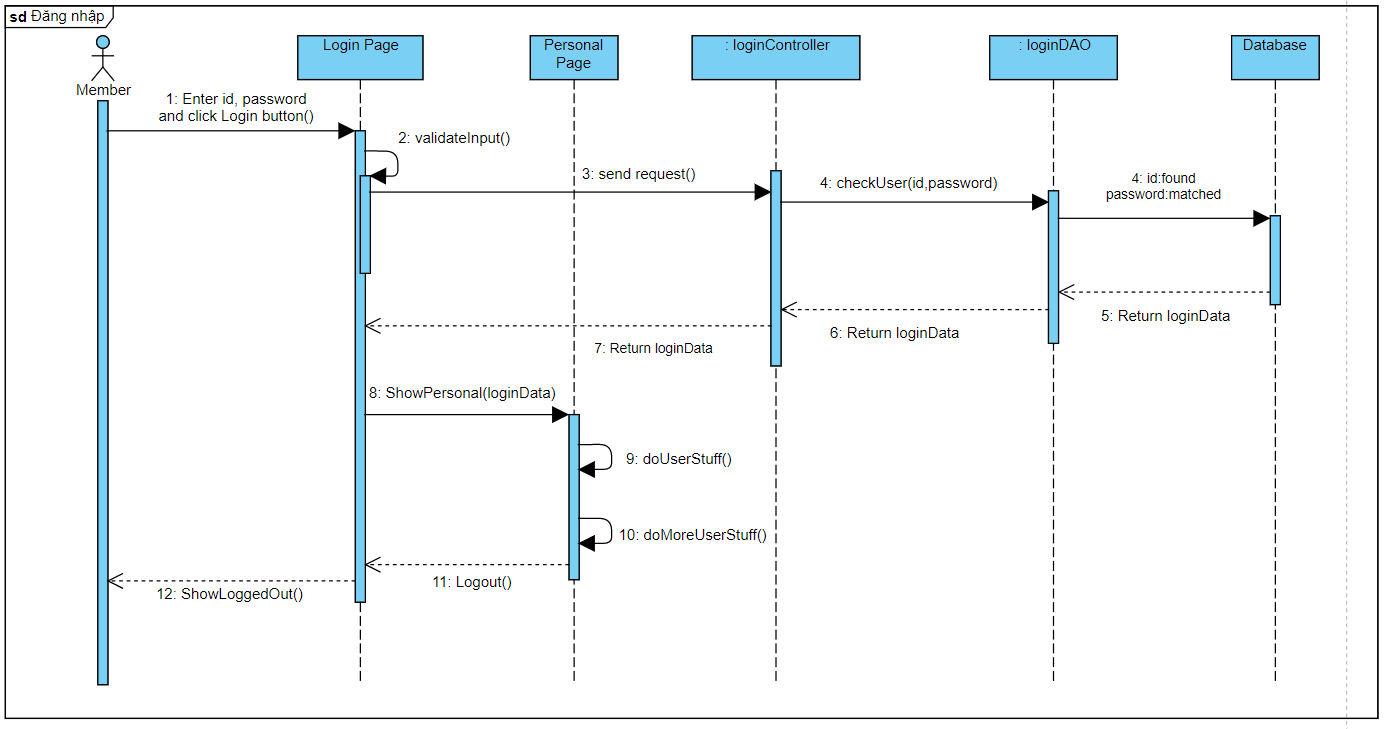
\includegraphics[scale=.45]{Hinh/Sequence diagram Đăng nhập.png}
		\end{center}
		\caption{Squence Diagram - Đăng nhập}
	\end{figure}
\end{center}

\pagebreak
\begin{center}
	\begin{figure}[!htp]
		\subsection{Sequence diagram - Lấy số thứ tự}
		\begin{center}
			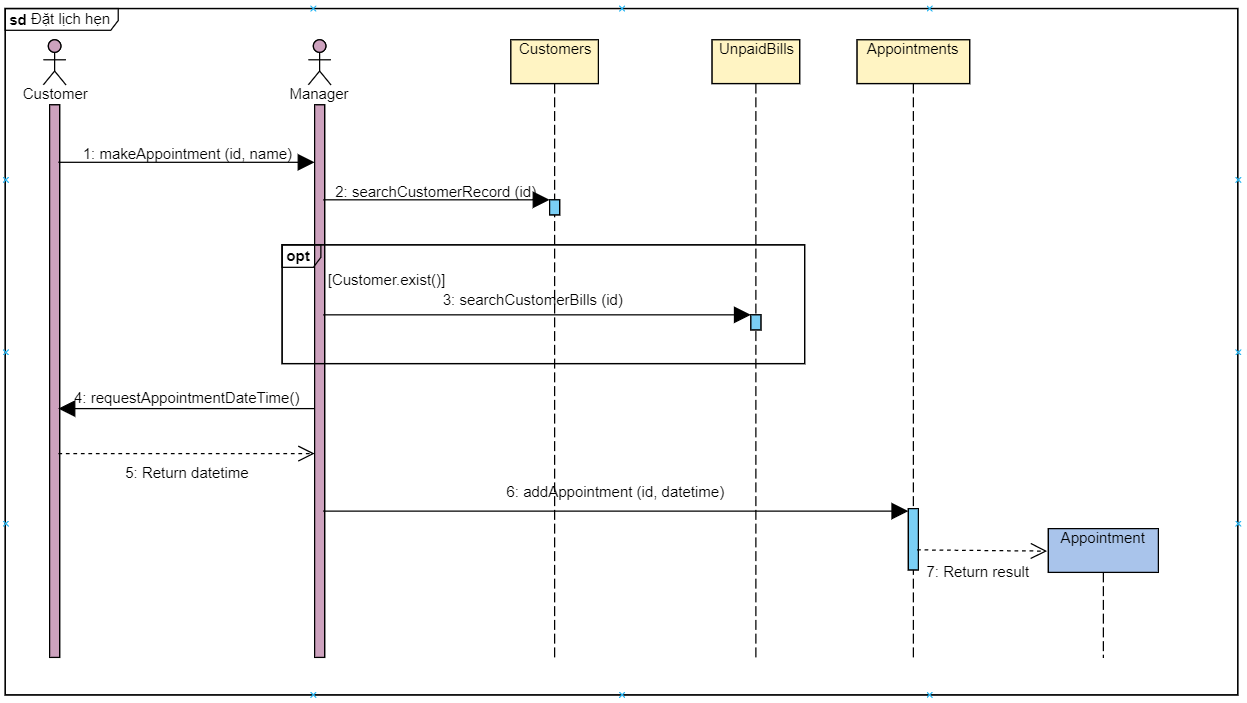
\includegraphics[scale=.5]{Hinh/Sequence diagram Lấy số thứ tự.png}
		\end{center}
		\caption{Sequence diagram - Lấy số thứ tự}
	\end{figure}
\end{center}


\pagebreak
\begin{center}
	\begin{figure}[!htp]
		\subsection{Sequence diagram - Liên hệ hỏi đáp}
		\begin{center}
			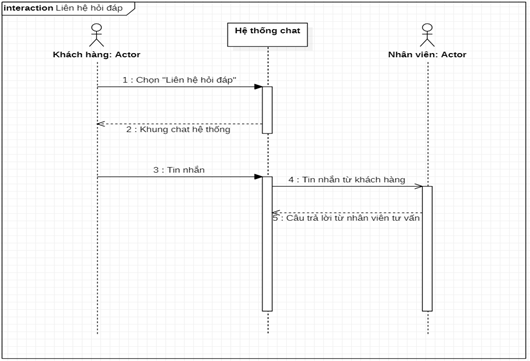
\includegraphics[scale=1]{Hinh/Sequence diagram Liên hệ hỏi đáp.png}
		\end{center}
		\caption{Sequence diagram - Liên hệ hỏi đáp}
	\end{figure}
\end{center}

\begin{center}
	\begin{figure}[!htp]
		\subsection{Sequence diagram - Tìm kiếm thông tin bệnh nhân}
		\begin{center}
			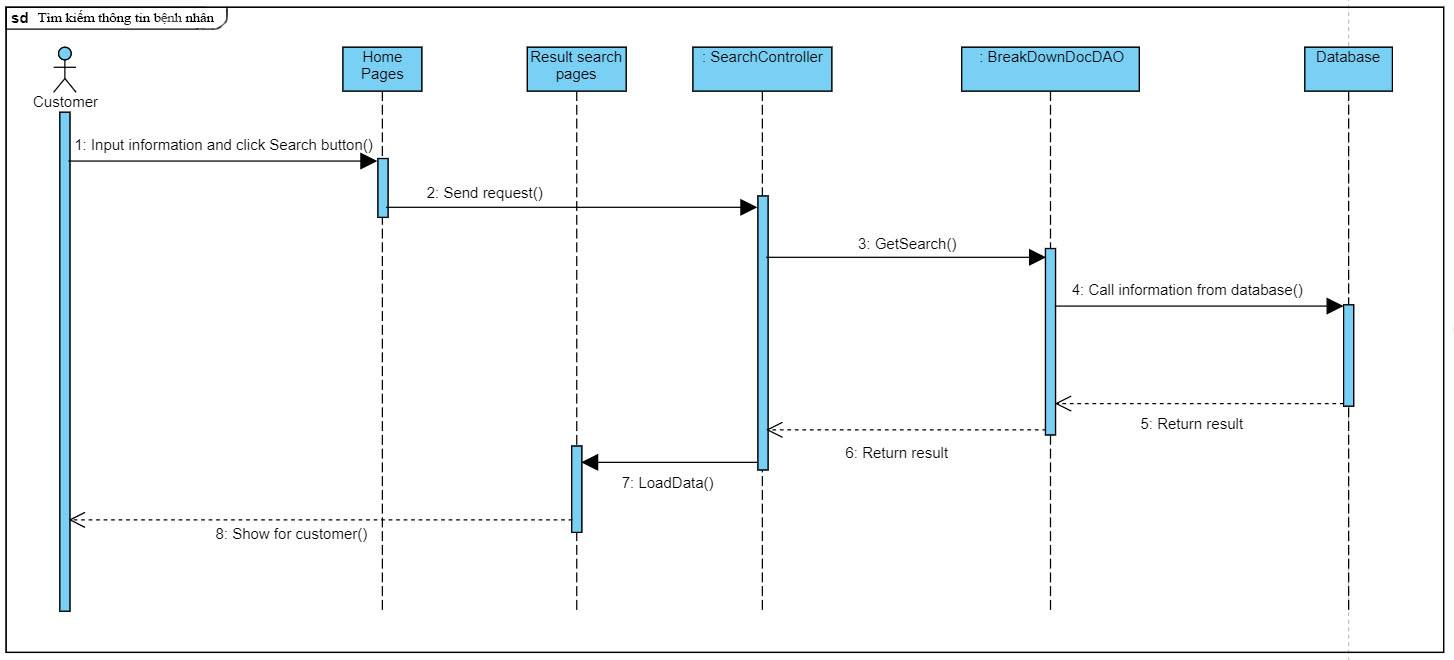
\includegraphics[scale=.3]{Hinh/Sequence diagram Tìm kiếm thông tin bệnh nhân.jpg}
		\end{center}
		\caption{Sequence diagram - Tìm kiếm thông tin bệnh nhân}
	\end{figure}
\end{center}

\pagebreak
\begin{center}
	\begin{figure}[!htp]
		\subsection{Sequence diagram - Thanh toán viện phí}
		\begin{center}
			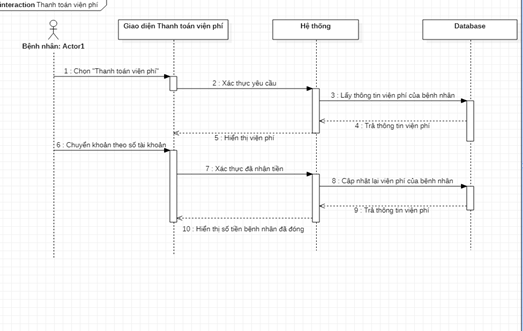
\includegraphics[scale=1]{Hinh/Sequence diagram Thanh toán viện phí.png}
		\end{center}
		\caption{Sequence diagram - Thanh toán viện phí}
	\end{figure}
\end{center}

\begin{center}
	\begin{figure}[!htp]
		\subsection{Sequence diagram - Xem thông tin, hoạt động phòng khám}
		\begin{center}
			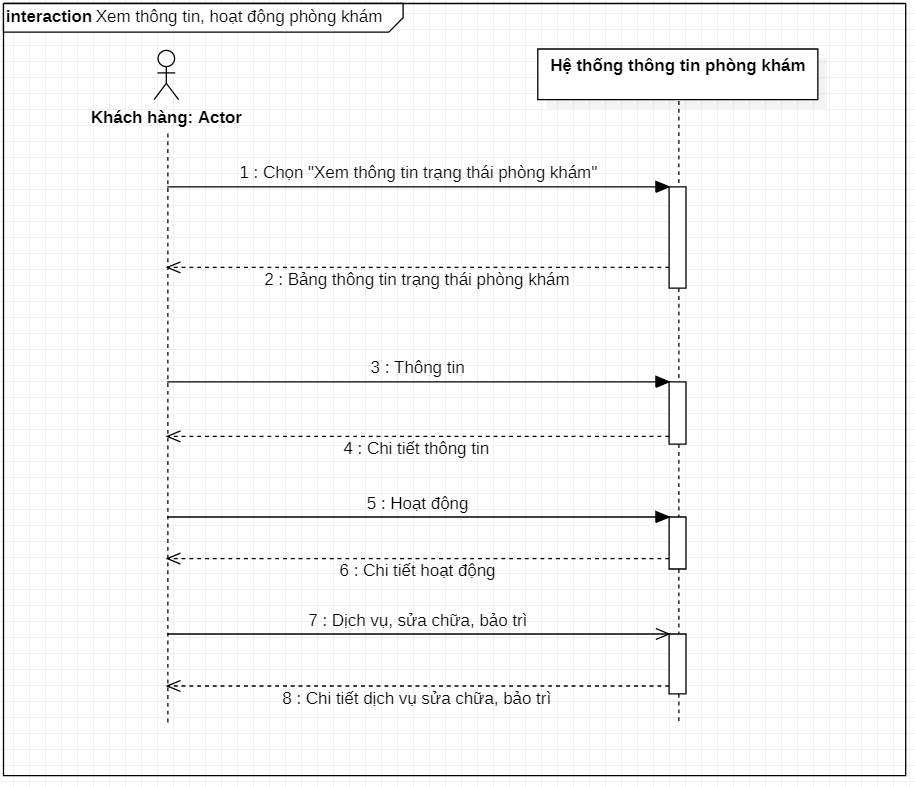
\includegraphics[scale=.35]{Hinh/Sequence diagram Xem thông tin, hoạt động phòng khám.png}
		\end{center}
		\caption{Sequence diagram - Xem thông tin, hoạt động phòng khám}
	\end{figure}
\end{center}

\begin{center}
	\begin{figure}[!htp]
		\subsection{Sequence diagram - Xem tổng quát và chi tiết tất cả hồ sơ bệnh án}
		\begin{center}
			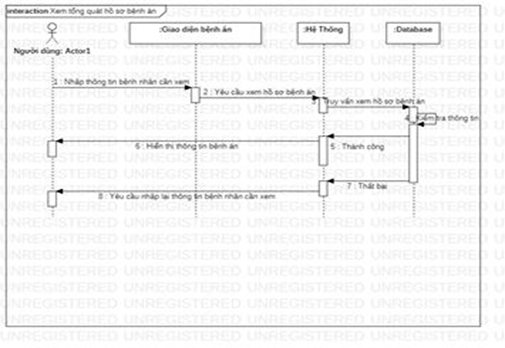
\includegraphics[scale=1]{Hinh/Sequence diagram Xem tổng quát và chi tiết tất cả hồ sơ bệnh án.png}
		\end{center}
		\caption{Sequence diagram - Xem tổng quát và chi tiết tất cả hồ sơ bệnh án}
	\end{figure}
\end{center}

\pagebreak
\begin{center}
	\begin{figure}[!htp]
		\subsection{Sequence diagram - Xem hồ sơ bệnh án}
		\begin{center}
			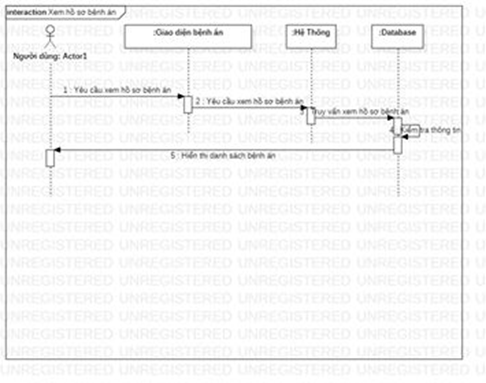
\includegraphics[scale=1]{Hinh/Sequence diagram Xem hồ sơ bệnh án.png}
		\end{center}
		\caption{Sequence diagram - Xem hồ sơ bệnh án}
	\end{figure}
\end{center}

\begin{center}
	\begin{figure}[!htp]
		\subsection{Sequence diagram - Cập nhật hồ sơ bệnh nhân}
		\begin{center}
			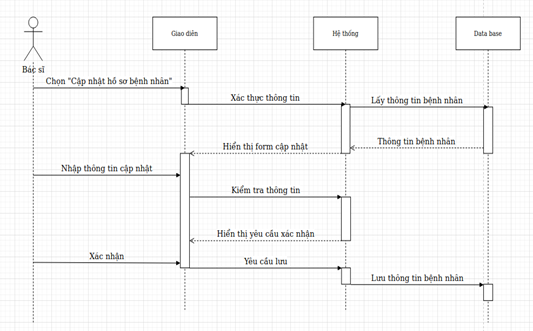
\includegraphics[scale=1.1]{Hinh/Sequence diagram Cập nhật hồ sơ bệnh nhân.png}
		\end{center}
		\caption{Sequence diagram - Cập nhật hồ sơ bệnh nhân}
	\end{figure}
\end{center}

\pagebreak
\begin{center}
	\begin{figure}[!htp]
		\subsection{Sequence diagram - Xem thông tin kho thuốc}
		\begin{center}
			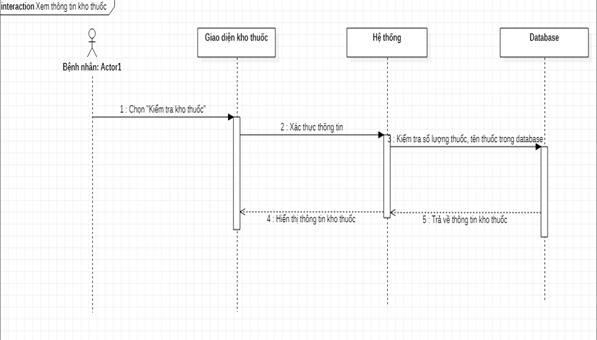
\includegraphics[scale=1]{Hinh/Sequence diagram Xem thông tin kho thuốc.png}
		\end{center}
		\caption{Sequence diagram - Xem thông tin kho thuốc}
	\end{figure}
\end{center}

\begin{center}
	\begin{figure}[!htp]
		\subsection{Sequence diagram - Thống kê kho thuốc}
		\begin{center}
			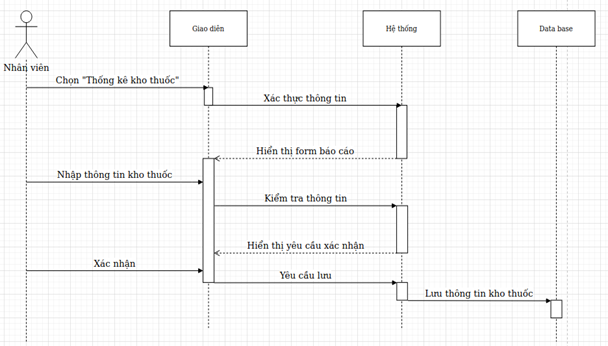
\includegraphics[scale=1]{Hinh/Sequence diagram Thống kê kho thuốc.png}
		\end{center}
		\caption{Sequence diagram - Thống kê kho thuốc}
	\end{figure}
\end{center}

\pagebreak
\begin{center}
	\begin{figure}[!htp]
		\subsection{Sequence diagram - Nhập kho thuốc}
		\begin{center}
			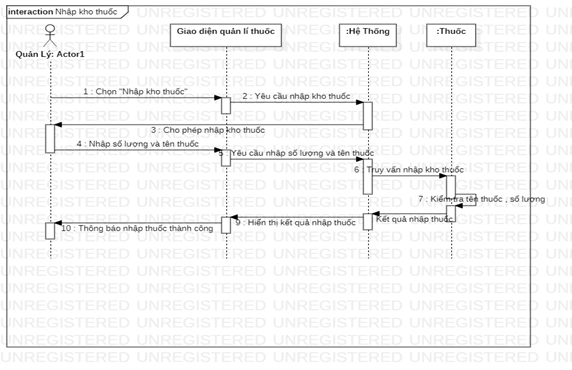
\includegraphics[scale=1]{Hinh/Sequence diagram Nhập kho thuốc.png}
		\end{center}
		\caption{Sequence diagram - Nhập kho thuốc}
	\end{figure}
\end{center}

\pagebreak
\begin{center}
	\begin{figure}[!htp]
		\subsection{Sequence diagram - Xuất kho trả}
		\begin{center}
			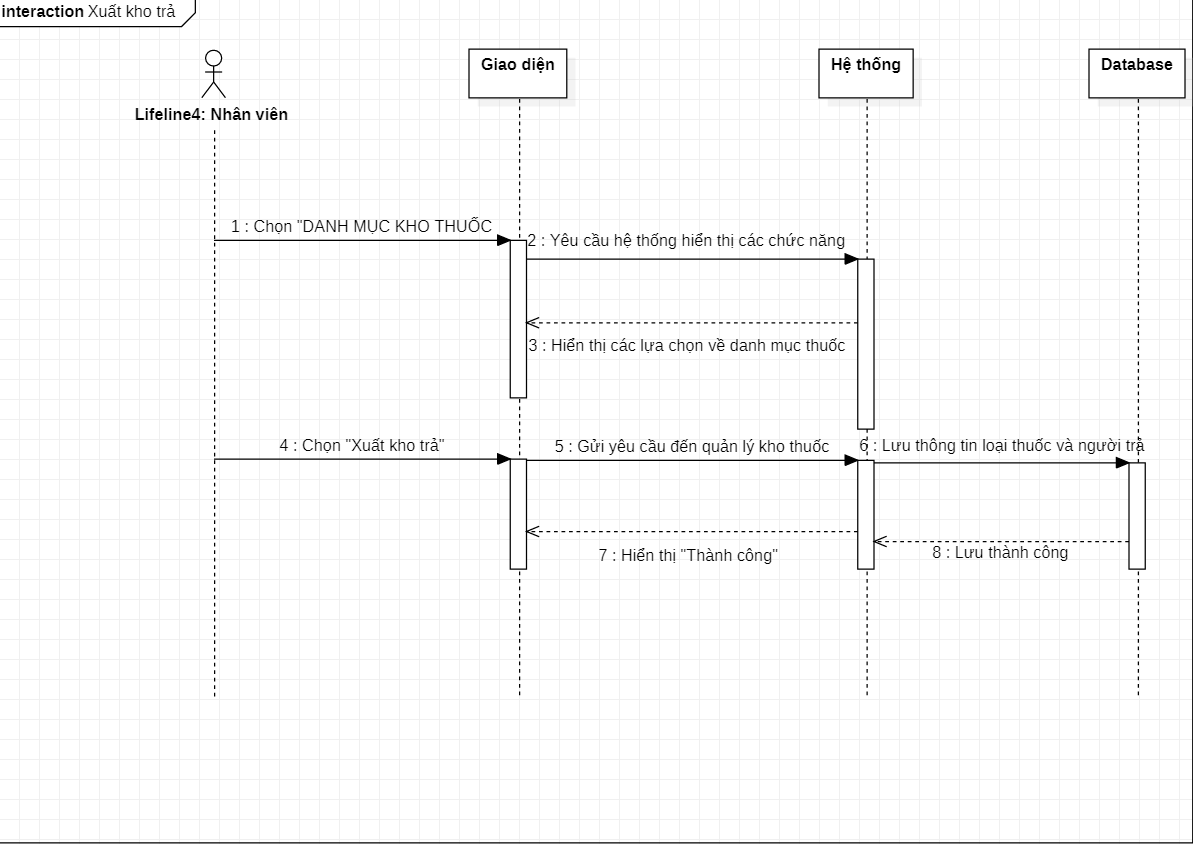
\includegraphics[scale=.4]{Hinh/Sequence diagram Xuất kho trả.png}
		\end{center}
		\caption{Sequence diagram - Xuất kho trả}
	\end{figure}
\end{center}

\pagebreak
\begin{center}
	\begin{figure}[!htp]
		\subsection{Sequence diagram - Xuất kho hủy}
		\begin{center}
			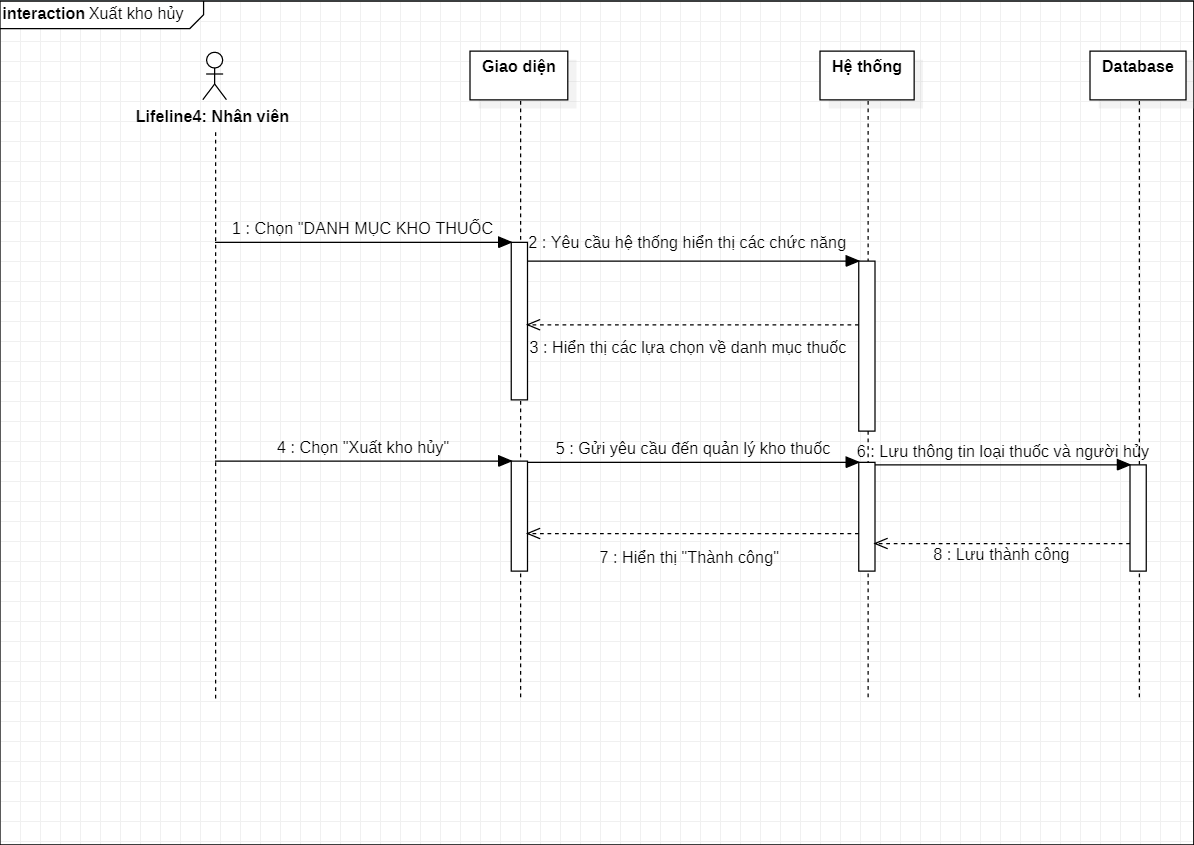
\includegraphics[scale=.35]{Hinh/Sequence diagram Xuất kho hủy.png}
		\end{center}
		\caption{Sequence diagram - Xuất kho hủy}
	\end{figure}
\end{center}

\begin{center}
	\begin{figure}[!htp]
		\subsection{Sequence diagram - Báo cáo}
		\begin{center}
			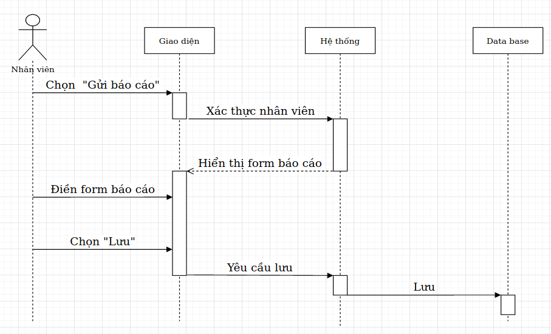
\includegraphics[scale=.8]{Hinh/Sequence diagram Báo cáo.png}
		\end{center}
		\caption{Sequence diagram - Báo cáo}
	\end{figure}
\end{center}

\begin{center}
	\begin{figure}[!htp]
		\subsection{Sequence diagram - Xem thông tin người dùng}
		\begin{center}
			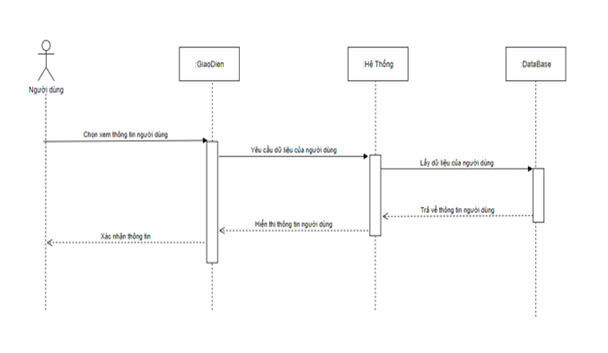
\includegraphics[scale=1]{Hinh/Sequence diagram Xem thông tin người dùng.png}
		\end{center}
		\caption{Sequence diagram - Xem thông tin người dùng}
	\end{figure}
\end{center}

\pagebreak
\begin{center}
	\begin{figure}[!htp]
		\subsection{Sequence diagram - Tạo tài khoản nhân viên}
		\begin{center}
			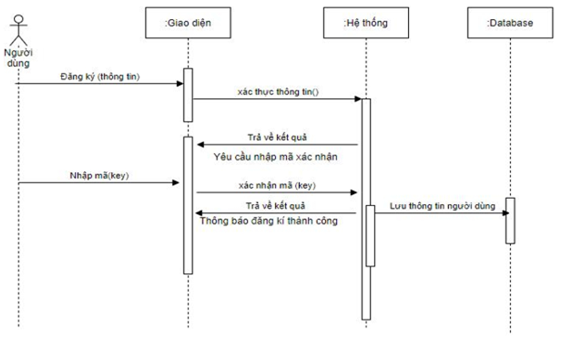
\includegraphics[scale=1]{Hinh/Sequence diagram Tạo tài khoản nhân viên.png}
		\end{center}
		\caption{Sequence diagram - Tạo tài khoản nhân viên}
	\end{figure}
\end{center}

\pagebreak
\begin{center}
	\begin{figure}[!htp]
		\subsection{Sequence diagram - Xóa thông tin người dùng}
		\begin{center}
			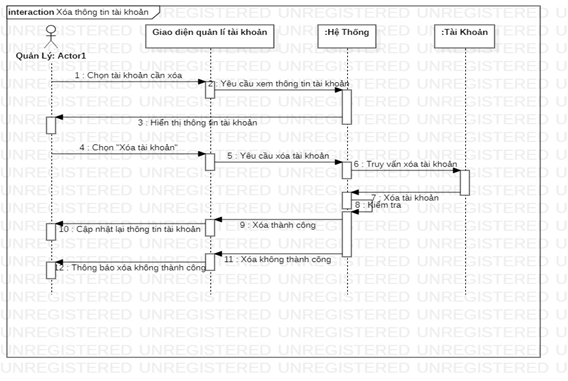
\includegraphics[scale=1]{Hinh/Sequence diagram Xóa thông tin người dùng.png}
		\end{center}
		\caption{Sequence diagram - Xóa thông tin người dùng}
	\end{figure}
\end{center}

\pagebreak
\begin{center}
	\begin{figure}[!htp]
		\subsection{Sequence diagram - Sửa thông tin người dùng}
		\begin{center}
			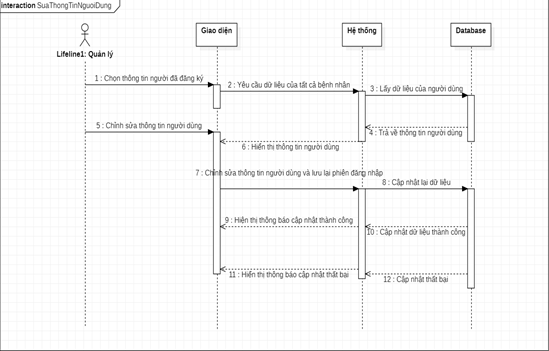
\includegraphics[scale=1]{Hinh/Sequence diagram Sửa thông tin người dùng.png}
		\end{center}
		\caption{Sequence diagram - Sửa thông tin người dùng}
	\end{figure}
\end{center}

\pagebreak
\section{Class Diagram}
\begin{center}
	\begin{figure}[!htp]
		\begin{center}
			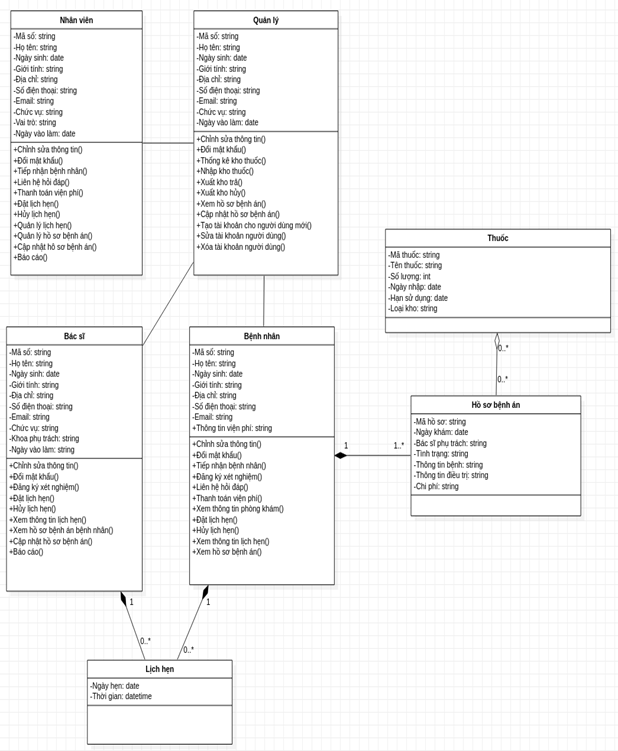
\includegraphics[scale=.9]{Hinh/Class diagram.png}
		\end{center}
		\caption{Class Diagram}
	\end{figure}
\end{center}

\pagebreak
\section{Sơ đồ quan hệ - thực thể (Entity - Relationship Diagram) }
\begin{center}
	\begin{figure}[!htp]
		\subsection{Sơ đồ ERD}
		\begin{center}
			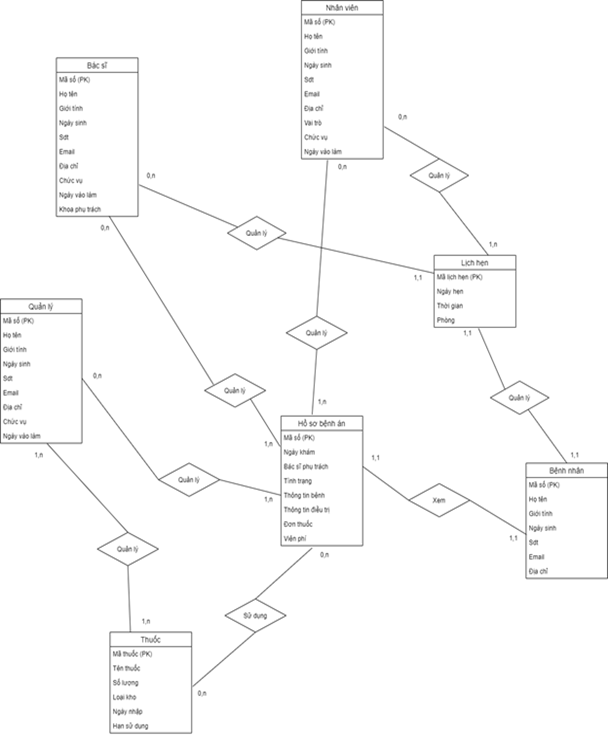
\includegraphics[scale=1]{Hinh/ERD.png}
		\end{center}
		\caption{Sơ đồ ERD}
	\end{figure}
\end{center}

\pagebreak
\subsection{Sơ đồ ERD sang mô hình quan hệ}
\paragraph{}
· BacSi(MaBacSi, HoTen, GioiTinh, NgaySinh, SDT, Email, DiaChi, Chuc Vu, NgayVaoLam, Khoa Phu Trach)
\paragraph{}
· NhanVien(MaNhanVien, HoTen, GioiTinh, NgaySinh, SDT, Email, DiaChi, Vai Tro, Chuc Vu, NgayVaoLam)
\paragraph{}
· QuanLy(MaQuanLy, HoTen, GioiTinh, NgaySinh, SDT, Email, DiaChi, ChucVu, NgayVaoLam)
\paragraph{}
· HoSoBenhAn(MaHoSo, Ngay Kham, Bac Si Phu Trach, TinhTrang, Thong Tin Benh, ThongTin Dieu Tri, Don Thuoc, VienPhi)
\paragraph{}
· LichHen(MaLichHen, NgayHen, ThoiGian, Phong)
\paragraph{}
· BenhNhan(MaBenhNhan, HoTen, GioiTinh, NgaySinh, SDT, Email, DiaChi)
\paragraph{}
· Thuoc(MaThuoc, TenThuoc, SoLuong, LoaiKho, NgayNhap, HSD)




\pagebreak
\raggedright
\section{State Machine Diagram}
\begin{center}
	\begin{figure}[!htp]
		\subsection{State Machine diagram - Thuốc}
		\begin{center}
			\includegraphics[scale=.9]{Hinh/State Machine diagram Thuốc.png}
		\end{center}
		\caption{State Machine diagram - Thuốc}
	\end{figure}
\end{center}

\begin{center}
	\begin{figure}[!htp]
		\subsection{State Machine diagram - Hồ sơ bệnh án}
		\begin{center}
			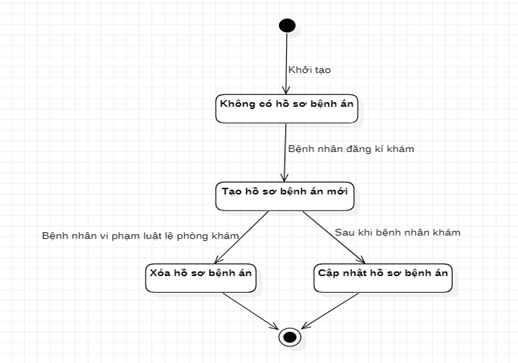
\includegraphics[scale=.9]{Hinh/State Machine diagram Hồ sơ bệnh án.png}
		\end{center}
		\caption{State Machine diagram - Hồ sơ bệnh án}
	\end{figure}
\end{center}


\begin{center}
	\begin{figure}[!htp]
		\subsection{State Machine diagram - Đăng nhập}
		\begin{center}
			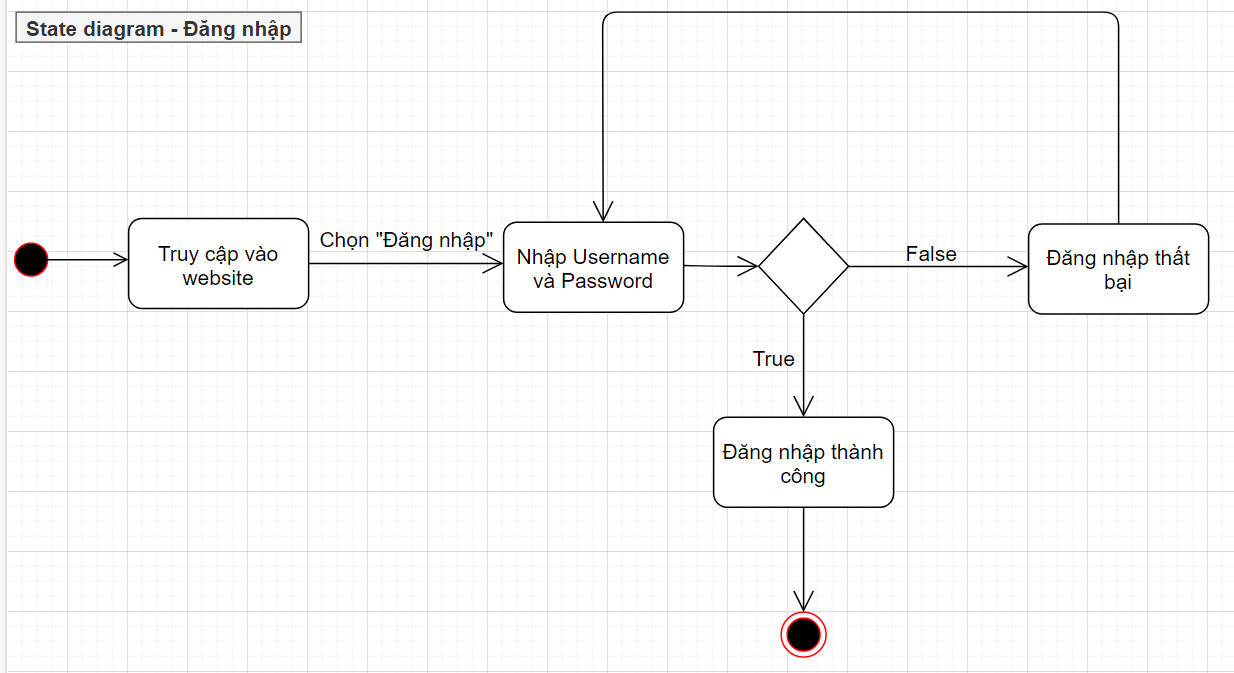
\includegraphics[scale=.5]{Hinh/State Machine diagram Đăng nhập.png}
		\end{center}
		\caption{State Machine diagram - Đăng nhập}
	\end{figure}
\end{center}

\pagebreak
\begin{center}
	\begin{figure}[!htp]
		\subsection{State Machine diagram - Tìm kiếm thông tin bệnh nhân}
		\begin{center}
			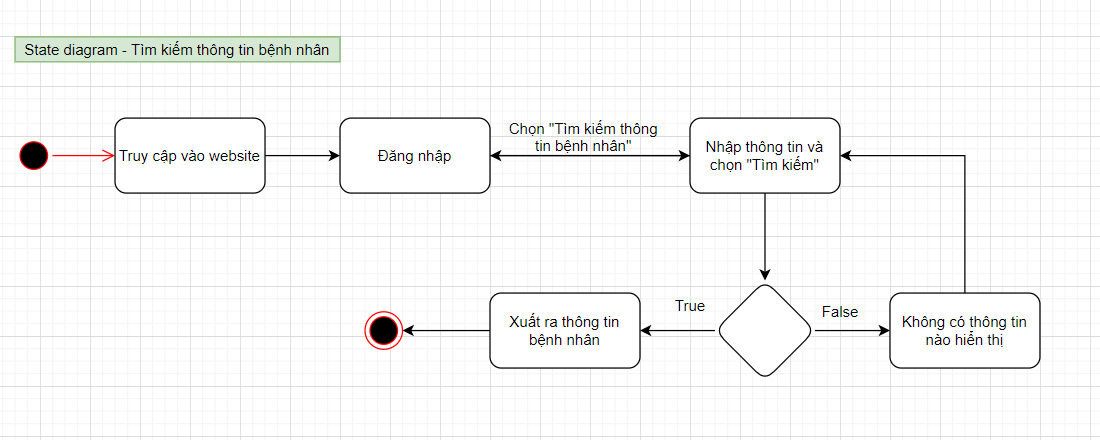
\includegraphics[scale=.6]{Hinh/State Machine diagram Tìm kiếm thông tin bệnh nhân.png}
		\end{center}
		\caption{State Machine diagram - Tìm kiếm thông tin bệnh nhân}
	\end{figure}
\end{center}


\pagebreak
\section{Activity Diagram}
\begin{center}
	\begin{figure}[!htp]
		\subsection{Activity Diagram - Tiếp nhận và ghi nhận thông tin bệnh nhân}
		\begin{center}
			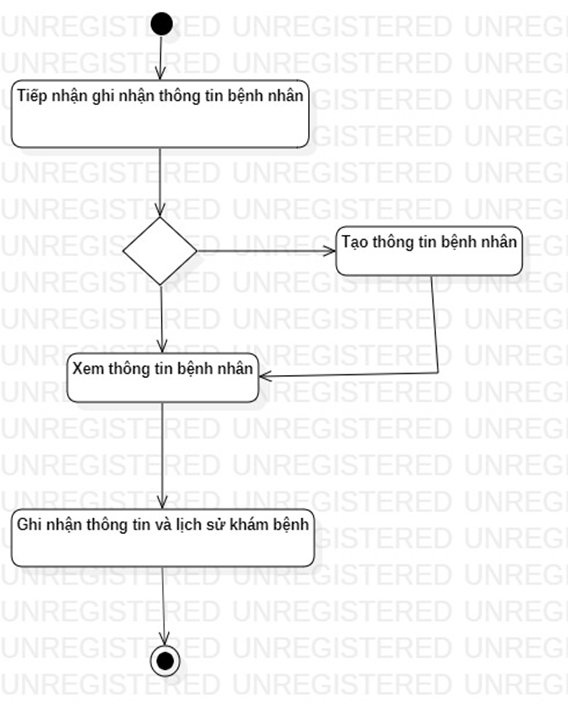
\includegraphics[scale=1]{Hinh/Activity diagram Tiếp nhận và ghi nhận thông tin bệnh nhân.png}
		\end{center}
		\caption{Activity Diagram - Tiếp nhận và ghi nhận thông tin bệnh nhân}
	\end{figure}
\end{center}

\begin{center}
	\begin{figure}[!htp]
		\subsection{Activity Diagram - Đăng ký xét nghiệm}
		\begin{center}
			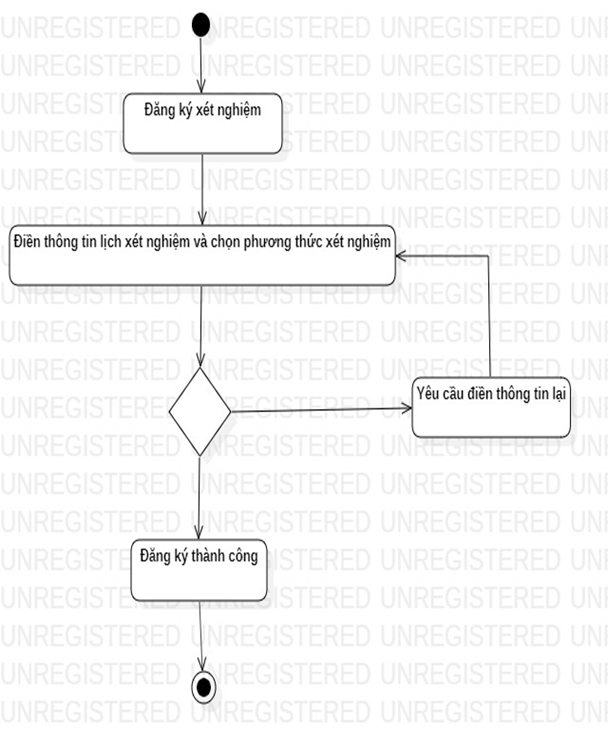
\includegraphics[scale=1]{Hinh/Activity diagram Đăng ký xét nghiệm.png}
		\end{center}
		\caption{Activity Diagram - Đăng ký xét nghiệm}
	\end{figure}
\end{center}

\begin{center}
	\begin{figure}[!htp]
		\subsection{Activity Diagram - Đăng nhập}
		\begin{center}
			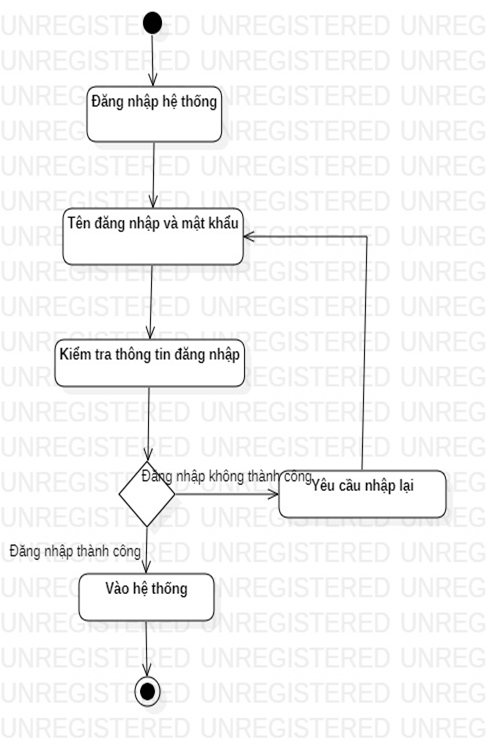
\includegraphics[scale=1]{Hinh/Activity diagram Đăng nhập.png}
		\end{center}
		\caption{Activity Diagram - Đăng nhập}
	\end{figure}
\end{center}


\begin{center}
	\begin{figure}[!htp]
		\subsection{Activity Diagram - Thanh toán viện phí}
		\begin{center}
			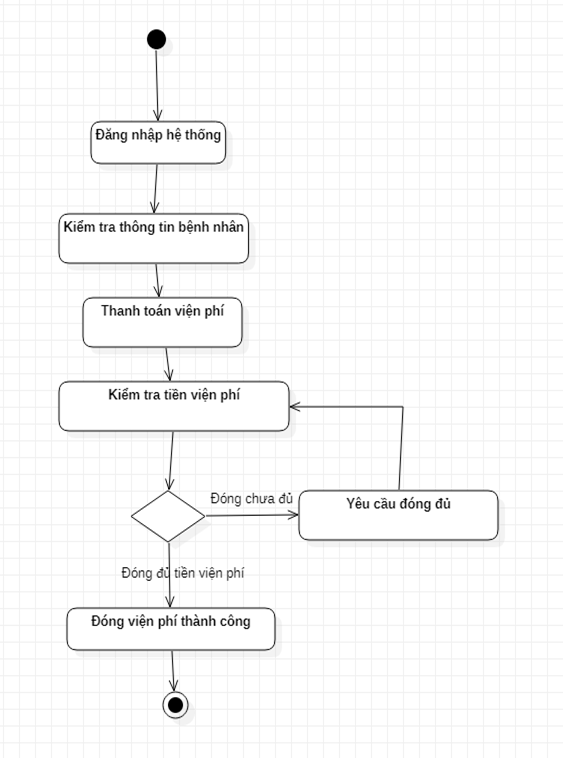
\includegraphics[scale=1]{Hinh/Activity diagram Thanh toán viện phí.png}
		\end{center}
		\caption{Activity Diagram - Thanh toán viện phí}
	\end{figure}
\end{center}

\begin{center}
	\begin{figure}[!htp]
		\subsection{Activity Diagram - Thống kê kho thuốc}
		\begin{center}
			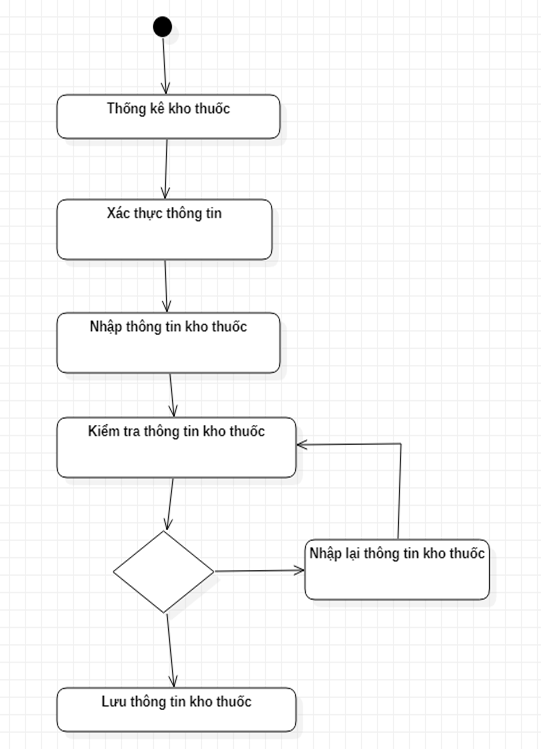
\includegraphics[scale=1]{Hinh/Activity diagram Thống kê kho thuốc.png}
		\end{center}
		\caption{Activity Diagram - Thống kê kho thuốc}
	\end{figure}
\end{center}

%--------------------------------------------------------
\chapter{TÀI LIỆU THAM KHẢO}
\fontsize{13}{15}\selectfont
\raggedright
\paragraph{}
[1]. J.W. Satzinger, R.B. Jackson, S.D. Burd, [2010], Object-Oriented Analysis and Design with the Unified Process, Course Technology, Boston.
\paragraph{}
[2]. Howard Podeswa, [2010], UML for the IT Business Analyst, Course Technology, Boston.
\paragraph{}
[3]. J.W. Satzinger, R.B. Jackson, S.D. Burd, [2011], Systems Analysis and Design in a Changing World, 6th edition, Course Technology, Australia.
\paragraph{}
[4]. TS Ngô Minh Vương, TS Nguyễn Thị Thanh Sang, TS Nguyễn Thành Sơn, TS Dương Thị Thùy Vân, [2017], Phân tích và thiết kế hệ thống thông tin, Đại học quốc gia Thành phố Hồ Chí Minh, Thành phố Hồ Chí Minh.
\end{document}

